% !TeX program = xelatex
\documentclass[UTF8,12pt,a4paper]{ctexart}
\usepackage{float}
\usepackage{enumitem}
\usepackage{listings}
\usepackage{xcolor}

\lstset{
  language=C++,
  basicstyle=\ttfamily\small,
  keywordstyle=\color{blue},
  commentstyle=\color{gray},
  stringstyle=\color{red},
  numbers=left,
  numberstyle=\tiny,
  stepnumber=1,
  numbersep=6pt,
  frame=single,
  breaklines=true,
  showstringspaces=false
}


% ================= 页面与行距 =================
\usepackage[a4paper,margin=2.5cm]{geometry}
\usepackage{setspace}
\onehalfspacing

% ================= 页眉页脚 =================
\usepackage{fancyhdr}
\usepackage{lastpage}

\pagestyle{fancy}
\fancyhf{} % 清空默认页眉页脚

% 页眉：左 固定文字；右 当前一级标题（section）
\fancyhead[L]{计算机网络课程设计}
\fancyhead[R]{\nouppercase{\leftmark}}

% 页脚：中间页码
\fancyfoot[C]{\thepage}

% 页眉页脚的线（可按需保留/去掉）
\renewcommand{\headrulewidth}{0.4pt}
\renewcommand{\footrulewidth}{0pt}

% 让 \leftmark 显示为 “一、课程的目的和任务” 这种（包含编号）
\renewcommand{\sectionmark}[1]{\markboth{\thesection\ #1}{}}

% 头部高度，避免 fancyhdr 报警告
\setlength{\headheight}{15pt}


% ================= 字体：中文宋体 + 英文新罗马 =================
\usepackage{fontspec}

% 中文：宋体（需要你上传 simsun.ttc 到项目根目录）
\setCJKmainfont[
  Path = ./,
  Extension = .ttc
]{simsun}

% 英文/数字：Times New Roman
\setmainfont{Times New Roman}

% 正文：小四
\AtBeginDocument{\zihao{-4}}

% ================= 标题样式与编号体系 =================
\usepackage{titlesec}

% ---------- 一级标题：一、二、三、（黑体） ----------
\renewcommand{\thesection}{\chinese{section}、}
\titleformat{\section}
  {\zihao{3}\heiti}
  {\thesection}{0.3em}{}

% ---------- 二级标题：2.1 / 2.2 / 2.3（黑体，小四） ----------
\renewcommand{\thesubsection}{\arabic{section}.\arabic{subsection}}
\titleformat{\subsection}
  {\zihao{-4}\heiti}
  {\thesubsection}{0.3em}{}

% ---------- 三级标题：2.1.1 / 2.1.2 ...（黑体，小四） ----------
\renewcommand{\thesubsubsection}{\thesubsection.\arabic{subsubsection}}
\titleformat{\subsubsection}
  {\zihao{-4}\heiti}
  {\thesubsubsection}{0.3em}{}

% 正文显示到三级标题
\setcounter{secnumdepth}{3}

\newcommand{\inlinebullet}[1]{\noindent{\zihao{-4} ● #1：}}


% ================= 目录标题：用 ctex 官方接口（保证严格居中） =================
\ctexset{
  contentsname = {目\ 录},
  contentsnameformat = \centering\zihao{3}\bfseries\heiti,
  contentsnameskip = 1em
}

% ================= 目录条目格式：用 tocloft（只管缩进/点线） =================
\usepackage{tocloft}

% 目录深度：显示到 subsubsection（2.1.1 那层）
\setcounter{tocdepth}{3}

% 点线密度（接近 Word）
\renewcommand{\cftdotsep}{1.5}

% 目录条目字体：一级加粗，其余不加粗（均小四）
\renewcommand{\cftsecfont}{\zihao{-4}\bfseries}
\renewcommand{\cftsecpagefont}{\zihao{-4}\bfseries}

\renewcommand{\cftsubsecfont}{\zihao{-4}}
\renewcommand{\cftsubsecpagefont}{\zihao{-4}}

\renewcommand{\cftsubsubsecfont}{\zihao{-4}}
\renewcommand{\cftsubsubsecpagefont}{\zihao{-4}}

% 目录缩进与“编号-标题”距离
\setlength{\cftsecindent}{0em}
% 注意：一级编号现在是“一、”，一般 1.8em 够；若后面有“十二、十三、”可适当调大
\setlength{\cftsecnumwidth}{0em}

\setlength{\cftsubsecindent}{1.5em}
\setlength{\cftsubsecnumwidth}{2.1em}

\setlength{\cftsubsubsecindent}{3.0em}
\setlength{\cftsubsubsecnumwidth}{2.8em}

% ================= 图表（备用） =================
\usepackage{graphicx}
\usepackage{caption}
\renewcommand{\figurename}{图}
\renewcommand{\tablename}{表}

\begin{document}

% ================= 封面（单独文件） =================
\begin{titlepage}
\centering

% ================= 顶部 left logo =================
% 尺寸：1.51cm × 9.84cm

\includegraphics[width=9.84cm]{logo_left.png}

\vspace{1.8cm}
\vspace{\baselineskip}
% ================= 标题（三号宋体加粗） =================
{\zihao{3}\bfseries 计算机网络课程设计报告\par}

\vspace{1.8cm}
\vspace{\baselineskip}
% ================= 下方 right logo =================
% 尺寸：5.11cm × 5.57cm

\includegraphics[width=5.11cm]{logo_right.png}

\vspace{2.5cm}

% ================= 个人信息区（内容压线） =================
\zihao{4}

\begin{tabular}{@{}l@{\quad}l@{}}
学\quad 号 &
\underline{\makebox[7.56cm][c]{XXXXXXXXXXXX}} \\[1.4em]

姓\quad 名 &
\underline{\makebox[7.56cm][c]{XXX}} \\[1.4em]

班\quad 级 &
\underline{\makebox[7.56cm][c]{XX学院XX专业XX班}} \\[1.4em]

提交日期 &
\underline{\makebox[7.56cm][c]{20XX年X月}}
\end{tabular}


\vfill
\end{titlepage}


% ================= 目录 =================
\tableofcontents
\newpage

% =================================================
% 一、课程的目的和任务
% =================================================
\section{课程的目的和任务}

\subsection{课程目标}

\begin{enumerate}[label=（\arabic*）, leftmargin=2em, itemsep=0.6em]
  \item 理解计算机网络体系结构和工作原理，掌握常用网络命令的功能，能够分析命令执行结果，
        运用常用网络命令进行网络测试与故障检测，并得到合理有效的结论。
  \item 能够进行网络组网设计，配置交换机和路由器，按照实验方案实施仿真实验，
        采集和整理实验数据，并对实验数据进行分析、处理和解释。
  \item 具备网络编程能力，能够进行简单网络编程，掌握设计协议分析程序的方法。
  \item 具备自主学习和创新意识，具有不断学习和适应技术发展的能力。
\end{enumerate}

\subsection{课程思政}

\begin{enumerate}[label=（\arabic*）, leftmargin=2em, itemsep=0.6em]
  \item 构建方案应立足实践基础，勇于创新和尝试，通过不断优化与迭代，实现精益求精。
  \item 尊重科学，实事求是。对于所设计的方案，能够通过实验进行验证，
        注重理论与实践相结合。
  \item 强化团结协作意识和责任担当精神，增强责任心与使命感。
\end{enumerate}

 
\subsection{课程任务}
 任务一、运用网络命令进行网络故障检测分析。掌握计算机网络相关命令原理及应用。常用网络命令ipconfig, ping, netstat, tracert, arp, telnet的功能；在windows环境下使用上述网络命令进行网络状态监测和跟踪，给出相应的截图和对结果的解释。

 任务二、基于交换机命令学习及交换机初始化设置的特定任务需求，构建系统方案、实施实验、处理数据并分析实验结果。基于交换机VLAN设置的特定任务需求，构建系统方案、实施实验、处理数据并分析实验结果。基于路由器端口、路由器命令学习和路由器登录方法的特定任务需求，构建系统方案、实施实验、并验证。基于静态路由、动态路由配置的特定任务需求，构建系统方案、实施实验、处理数据并分析实验结果。
 
 (1) 安装packet tracer，在packet tracer仿真环境下，熟悉交换机命令、交换机初始化配置；
 
 (2) 在交换机上实现VLAN配置；
 
 要求：创建三个VLAN，给出拓扑，查看VLAN信息
 
 (3) 基于Console控制台登录配置路由器，学习路由器配置相关命令；
 
 (4) 基于packet tracer构建网络环境，分别进行静态路由配置和基于RIP的动态路由配置，设计基于OSPF的动态路由配置。能够进行综合集成网络情景设计更佳。

 任务三、基于网络编程的特定任务需求进行socket编程，设计处理流程、数据结构、实施实验并分析实验结果。
 编程要求：捕获本机网卡的IP包，对捕获的IP包进行解析。要求必须输出以下字段：版本号、总长度、标志位、片偏移、协议、源地址和目的地址。
 
 要求有详细的说明文档，包括程序的设计思想、工作流程、关键问题、程序注释和对捕获包的解析截图。
 
 编程语言不作要求，可使用自己熟悉的C、C++、java或C#等。

\newpage

% =================================================
% 二、课程的基本内容和要求
% =================================================
\section{课程的基本内容和要求}

% ---------- 2.1 常用网络命令 ----------
\subsection{常用网络命令}

\subsubsection{课程要求}
运用网络命令进行网络故障检测分析。掌握计算机网络相关命令原理及应
用。常用网络命令 ipconfig, ping, netstat, tracert, arp, telnet 的功能；在 windows 环境下使
用上述网络命令进行网络状态监测和跟踪，给出相应的截图和对结果的解释。


\subsubsection{ipconfig}
\noindent {\heiti 功能、参数及原理}

该命令可以查看本机网络适配器的相关信息，包括各网络适配器的型号、MAC 地址、IP 地址、子网掩码、默认网关及 IP 租用时间。该命令还可以用于查看和刷新 DNS 缓存，以及用于进行 DHCP 相关的配置。

通过执行 ipconfig /?，可以查看该命令的参数。

\begin{figure}[htbp]
  \centering
  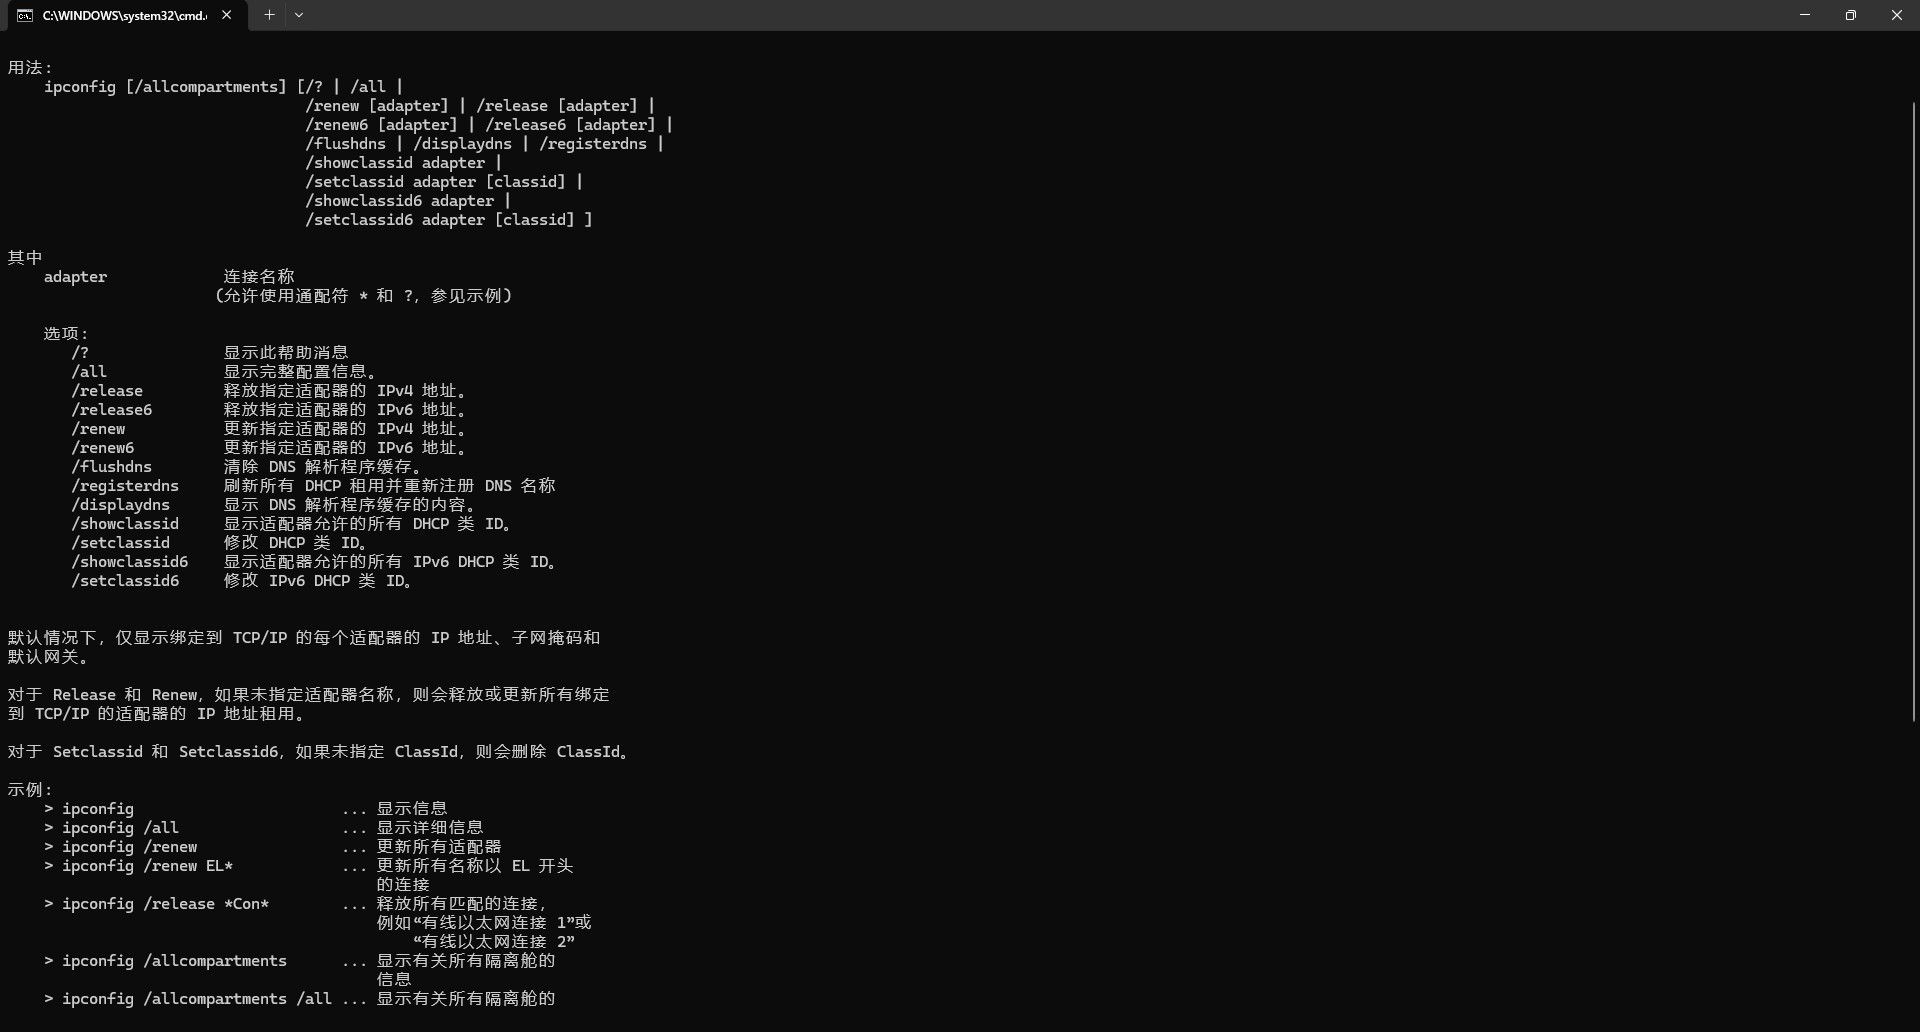
\includegraphics[width=1.0\textwidth]{figures/ipconfig.png}
  \caption{ipconfig /? 命令执行结果节选}
  \label{fig:jiwang}
\end{figure}


\noindent {\heiti 应用与分析}

接下来，我们将应用两个常见的命令，对其运行结果进行分析。

下图为执行 ipconfig /all 所得结果的节选，它描述了该本机无线网络适配器的配置信息。

\begin{figure}[H]
  \centering
  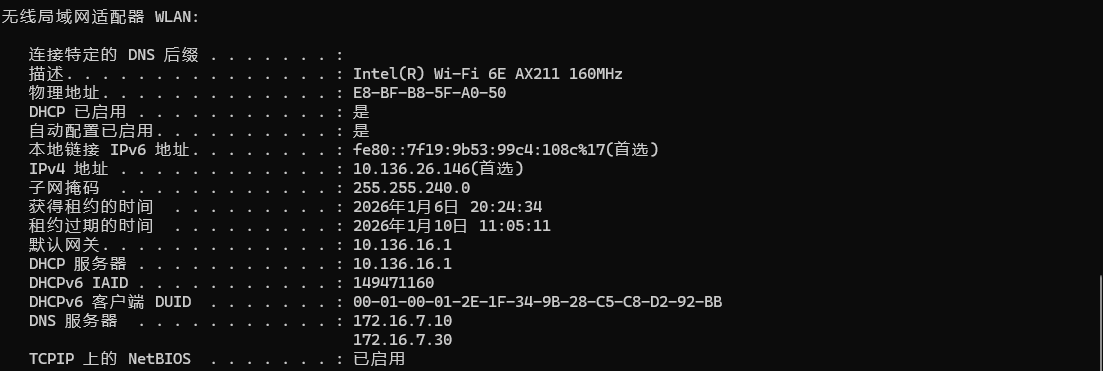
\includegraphics[width=1.0\textwidth]{figures/ipconfig_all.png}
  \caption{ipconfig /all 命令执行结果节选}
  \label{fig:jiwang}
\end{figure}

\inlinebullet{描述} 该网络适配器的型号为 Intel(R) Wi-Fi 6E AX211 160MHz。

\inlinebullet{物理地址} 该网络适配器的 MAC 地址为 E8-BF-B8-5F-A0-50。

\inlinebullet{DHCP 已启用} 该网络适配器已启用 DHCP，意味着允许使用 DHCP 自动获取 IP 地址。

\inlinebullet{IPv4 地址} 该网络适配器的首选 IPv4 地址为 10.136.26.146，其 IPv4 地址可以有多个，IPv6 地址同理。

\inlinebullet{子网掩码} 该网络适配器 IPv4 地址所对应的子网掩码为 255.255.240.0。

\inlinebullet{获得租约的时间} 和租约过期的时间表示由 DHCP 临时租用的 IP 地址的可用时间段。

\inlinebullet{默认网关} 该网络适配器 IPv4 地址所对应的默认网关为 10.136.16.1。

\inlinebullet{DNS 服务器} 该网络适配器所使用的 DNS 服务器为 10.136.16.1，可以有多个。

下图为执行 ipconfig /flushdns 所得的结果。通过这个命令，我们清除了本机 DNS 解析程序的缓存。DNS 缓存通过对一些 DNS 记录进行缓存，从而加速 DNS 查询的效率，我们还可以执行ipconfig /displaydns 来查看其缓存内容。

\begin{figure}[H]
  \centering
  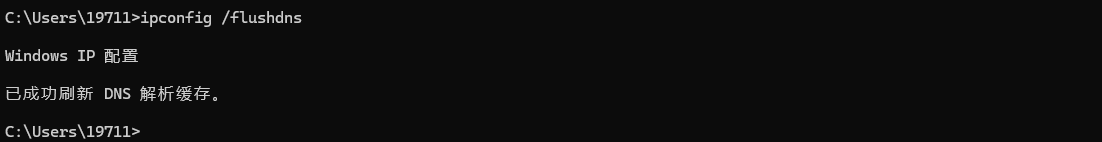
\includegraphics[width=1.0\textwidth]{figures/ipconfig_flushdns.png}
  \caption{ipconfig /flushdns 命令执行结果节选}
  \label{fig:jiwang}
\end{figure}

\subsubsection{ping}
\noindent {\heiti 功能、参数及原理}

该命令可以向指定主机发送 ICMP 请求报文，并返回数据包大小，往返时间，TTL 等，常用于检测本机与目的主机间是否可达。

通过执行 ping /?，可以查看该命令的参数。

\begin{figure}[H]
  \centering
  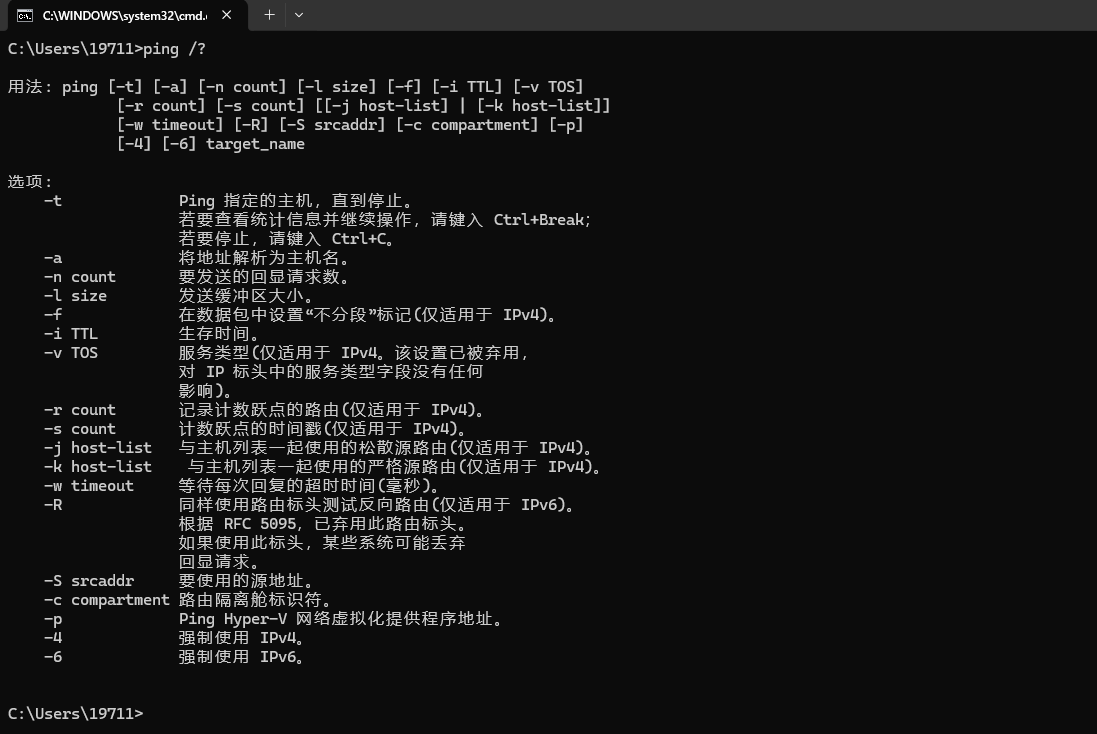
\includegraphics[width=1.0\textwidth]{figures/ping.png}
  \caption{ping /? 命令执行结果节选}
  \label{fig:jiwang}
\end{figure}

\noindent {\heiti 应用与分析}

接下来，我们加上一些参数执行 ping 命令。

如下图所示，我们执行 ping 10.136.26.164 -l 100 -n 4 ，向 ipconfig 命令查出的无线网络适配器 10.136.26.164 发送 4 个数据大小为 100 字节的数据包。

\begin{figure}[H]
  \centering
  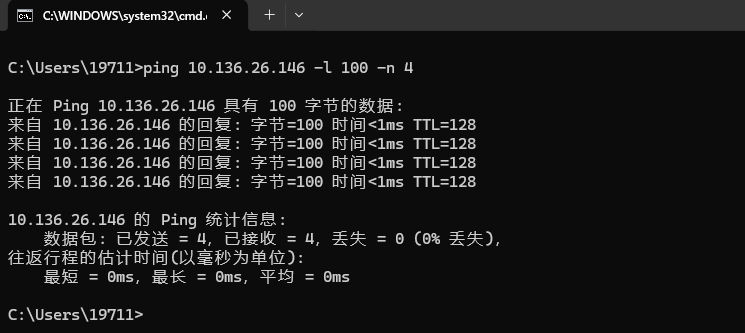
\includegraphics[width=1.0\textwidth]{figures/ping_dizhi.png}
  \caption{ping指定地址的执行结果}
  \label{fig:jiwang}
\end{figure}

所得结果我们可以看到，我们收到了来自 10.136.26.164的回复，耗时 0∼ 1ms。4个数据包都没有丢包，丢包率为 0\%，并且得到了最小、最大、平均 RTT。

TTL字段是指数据包的生存时间，ICMP包在网络中没转发一次，TTL就会减少 1，TTL的初始值与发送数据包的操作系统有关。目的地址 10.136.26.164为 Win10操作系统，通过查阅资料，其发送的响应 TTL为 128，由上图结果 TTL为 128，我们就可以推断响应数据包没有经过路由转发。

由于这个特性，在路由转发次数不是太多的情况下，我们可以用 ping命令大致确定目的地址的操作系统。

\subsubsection{netstat}
\noindent {\heiti 功能、参数与原理}

该命令可以查看在 TCP/IP网络连接下以太网信息、各协议的统计数据、路由表等，常用来查看和监听本机各端口的网络连接状况。

通过执行 netstat /?，可以查看该命令的参数。

\begin{figure}[H]
  \centering
  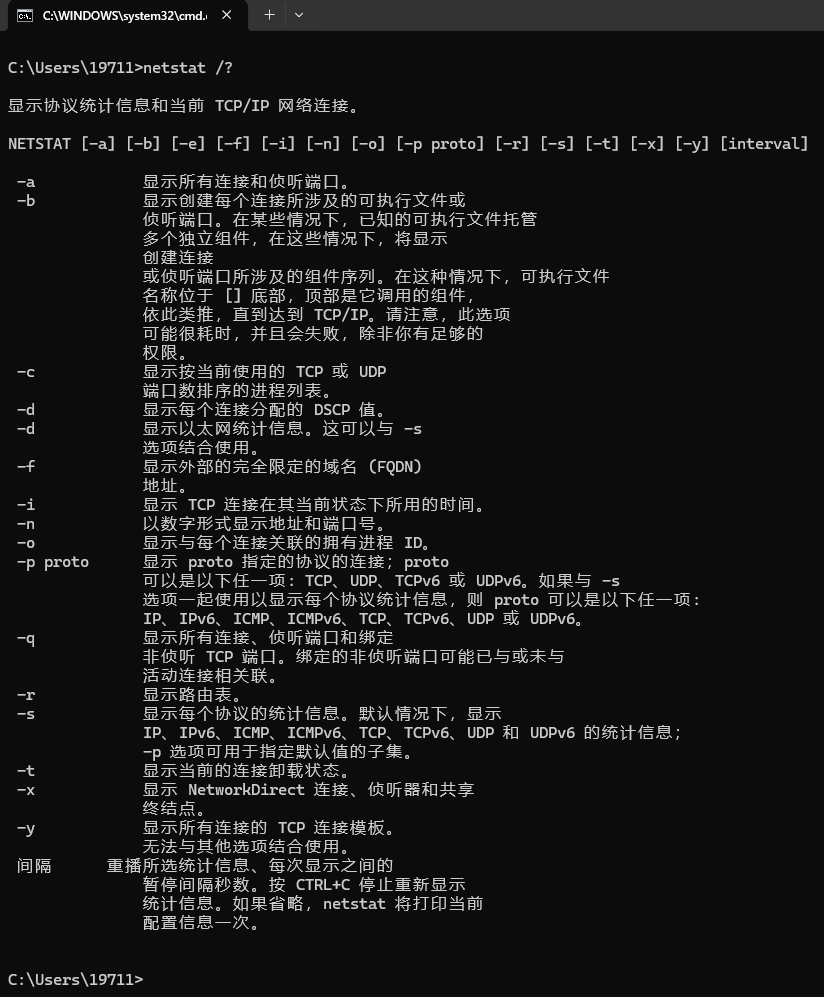
\includegraphics[width=0.8\textwidth]{figures/netstat.png}
  \caption{netstat /?执行结果}
  \label{fig:jiwang}
\end{figure}

\noindent {\heiti 应用与分析}

接下来，我们将应用两个常见的命令，对其运行结果进行分析。
首先，我们用 netstat -r查看本机路由表，运行结果如下图所示。

\begin{figure}[H]
  \centering
  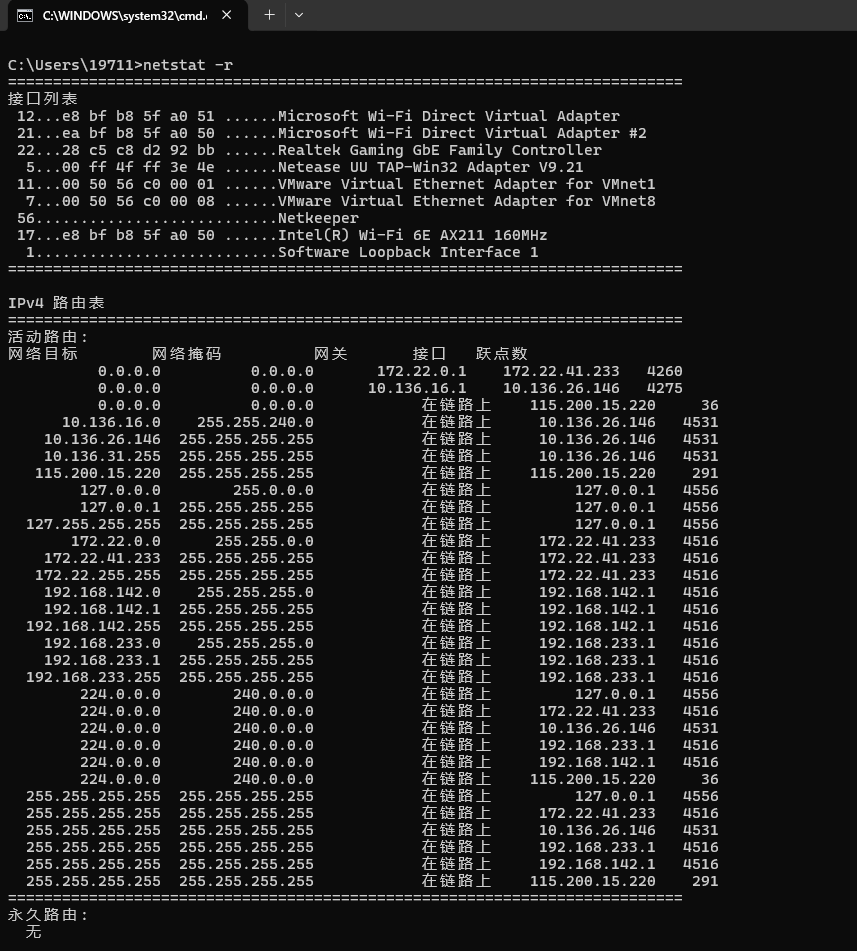
\includegraphics[width=0.8\textwidth]{figures/netstat_r.png}
  \caption{netstat -r 执行结果片段}
  \label{fig:jiwang}
\end{figure}

我们来分析一下路由表的各个字段：

\begin{itemize} %[leftmargin=*, itemsep=0.3em] % <- 有 enumitem 才能用这一行参数
  \item {\heiti 网络目标：} 即目的 IP 地址。结合本机路由表可见，
  存在默认路由（\texttt{0.0.0.0}），本机回环网段（\texttt{127.0.0.0}），
  受限广播地址（\texttt{255.255.255.255}）以及组播网段（\texttt{224.0.0.0}）。
  同时，本机还包含多个直连网络段，例如 \texttt{10.136.16.0/20}、
  \texttt{192.168.142.0/24} 与 \texttt{192.168.233.0/24} 等。

  \item {\heiti 网络掩码：} 用于与网络目标进行按位与运算，从而判断目的 IP 属于哪个网段；
  当存在多条可匹配路由时，通常遵循\textbf{最长前缀匹配}（掩码更长者优先）。

  \item {\heiti 网关：} 表示下一跳地址。由截图可见，本机存在两条默认路由：
  一条经网关 \texttt{172.22.41.233} 转发，另一条经网关 \texttt{10.136.16.1} 转发；
  而“在链路上”表示该目的网络为直连网络，无需经过下一跳。

  \item {\heiti 接口：} 表示该路由项对应的本机出接口（出站 IP）。
  例如默认路由可能从 \texttt{172.22.41.233} 或 \texttt{10.136.26.146} 出口转发；
  另外本机还存在虚拟网卡接口如 \texttt{192.168.142.1}、\texttt{192.168.233.1} 等。

  \item {\heiti 跃点数：} 反映路径代价（可理解为优先级/开销）。当多条路由同时满足匹配时，
  通常优先选择跃点数（Metric）较小的一条进行转发。
\end{itemize}

其次我们要分析的是 netstat最常见的应用，执行 netstat -a来查看端口占用情况和监听状态。我们添加参数将地址和端口号数字化，并指定所监听的协议为 TCP。执行 netstat -anp TCP结果如下图所示。

\begin{figure}[H]
  \centering
  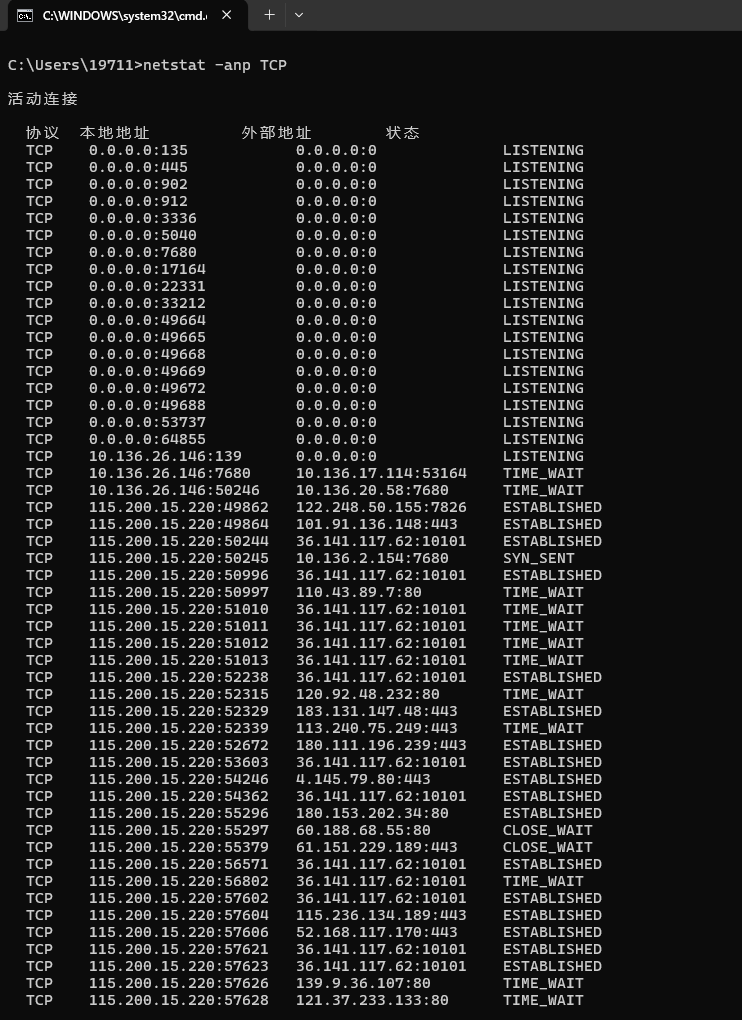
\includegraphics[width=0.8\textwidth]{figures/netstat_anc_TCP.png}
  \caption{netstat查看 TCP端口使用情况和监听状态执行结果}
  \label{fig:jiwang}
\end{figure}

我们可以看到协议为 TCP的监听端口和连接情况。我们对状态这一表项的各种取值举例分析：

\begin{itemize}
  \item {\heiti LISTENING：}
  表示本机正在监听某个 TCP 端口，等待远程主机发起连接。
  从截图可以看到，本机存在多个监听端口，
  例如 \texttt{0.0.0.0:5040}、\texttt{0.0.0.0:445} 等，
  其中 \texttt{0.0.0.0} 表示该端口在所有本地网络接口上监听。

  \item {\heiti ESTABLISHED：}
  表示 TCP 连接已经成功建立，通信双方可以正常进行数据传输。
  例如本机地址 \texttt{115.200.15.220} 的临时端口
  与远程主机 \texttt{183.131.147.48:443}、
  \texttt{180.111.196.239:443} 等建立了连接，
  根据端口号可以判断这些连接大多为 HTTPS 通信。

  \item {\heiti TIME\_WAIT：}
  表示本机已主动关闭连接，并发送了最后一个 ACK 报文，
  当前连接处于 TIME\_WAIT 状态。
  在该状态下，源 IP、源端口以及目的 IP、目的端口暂时不可复用，
  需要等待 \textbf{2MSL} 时间后，连接才会完全释放并转为 CLOSED 状态。

  \item {\heiti SYN\_SENT：}
  表示本机已向远程主机发送 SYN 报文，请求建立 TCP 连接，
  但尚未收到对方的 SYN+ACK 响应，说明连接仍处于建立过程中。

  \item {\heiti CLOSE\_WAIT：}
  表示远程主机已关闭连接，而本机尚未完成本地连接的关闭操作，
  通常需要等待应用程序关闭对应的套接字后，该状态才会消失。
\end{itemize}



\subsubsection{tracert}
\noindent {\heiti 功能、参数与原理}

tracert该命令通过发送带有不同 TLL的 ICMP数据包到目的地址来追踪经过的路由节点。TLL的原理在 ping命令中已经介绍过。

通过执行 tracert /?，可以查看该命令的参数。

\begin{figure}[H]
  \centering
  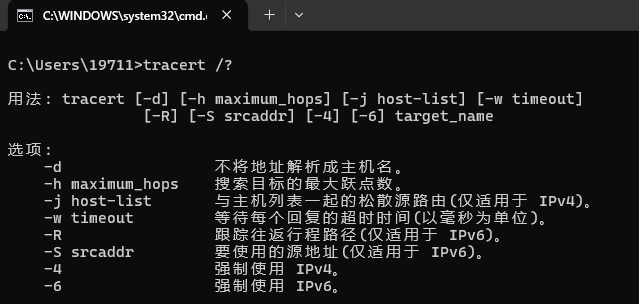
\includegraphics[width=0.8\textwidth]{figures/tracert.png}
  \caption{tracert /?命令执行结果}
  \label{fig:jiwang}
\end{figure}

在其基本功能的基础上，通过指定参数，我们可以指定最大路由跳数、超时时间等从而实现更加精准的网络诊断。

\noindent {\heiti 应用与分析}

我们对同一个无线网络下的另一台主机进行 tracert命令的测试。

\begin{figure}[H]
  \centering
  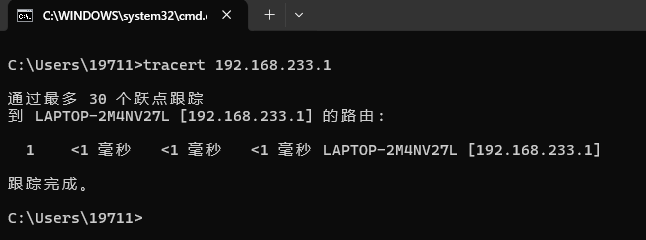
\includegraphics[width=0.8\textwidth]{figures/tracert_do.png}
  \caption{tracert 命令执行结果}
  \label{fig:jiwang}
\end{figure}

我们可以看到由于两台电脑属于同一个路由下的局域网，期间没有经过其它路由器转发。

\subsubsection{arp}
\noindent {\heiti 功能、参数与原理}

ARP协议通过解析 IP地址获取其对应的 MAC地址。arp命令可以让我们查看到本机的 ARP缓存内容，并且允许我们对 ARP缓存进行修改。

通过执行 arp /?，可以查看该命令的参数。

\begin{figure}[H]
  \centering
  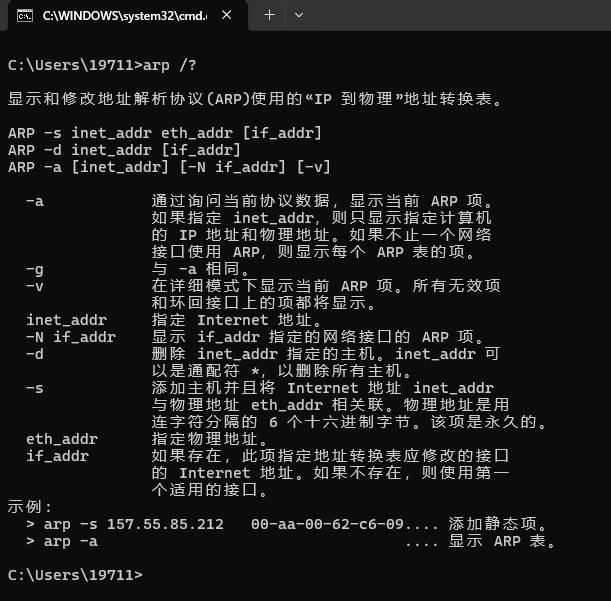
\includegraphics[width=0.65\textwidth]{figures/arp.png}
  \caption{arp /? 命令执行结果}
  \label{fig:jiwang}
\end{figure}

\noindent {\heiti 应用与分析}

我们执行 arp -a ，查看本机的 ARP 缓存内容，结果如下图所示。

\begin{figure}[H]
  \centering
  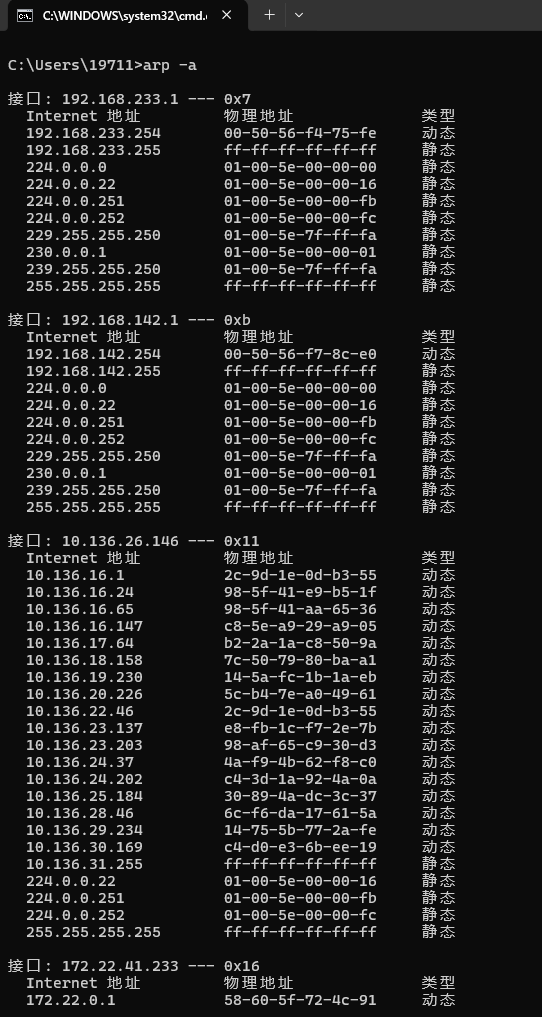
\includegraphics[width=0.6\textwidth]{figures/arp_a.png}
  \caption{arp 命令查看当前 ARP 缓存执行结果片段}
  \label{fig:jiwang}
\end{figure}

在上图中，有四个网络适配器，结合前面 ipconffg 的结果，可以知道第一个接口是无线网络的适配器。我们可以看到各个网络适配器中 IP 地址和 MAC 地址之间映射关系，类型 表项中 动态 表示该映射会定期向网络中询问并进行更新，静态 表示该映射不会自动进行更新。

\subsubsection{telnet}
\noindent {\heiti 功能、参数与原理}

该命令可以使 telnet 客户端进入 telnet 服务端的终端，常用于远程登录和控制服务器。

由于 telnet 在 Win10 中并默认是关闭的，我们需要在「控制面板」中的「打开或关闭 Windows功能」中将其客户端打开。

\begin{figure}[H]
  \centering
  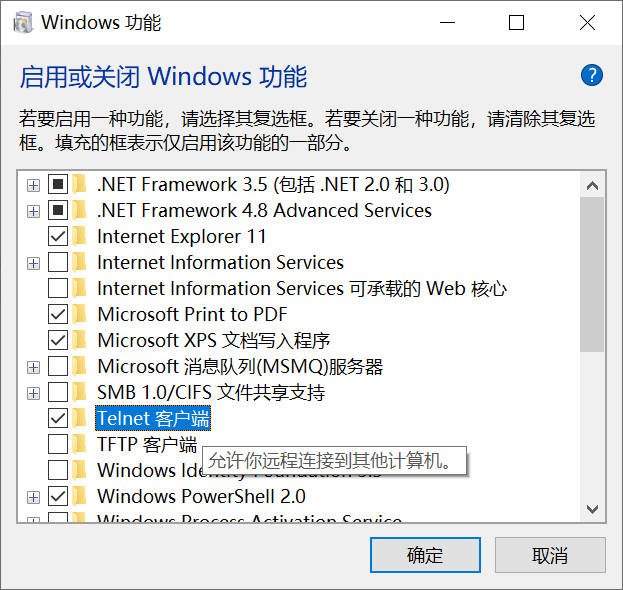
\includegraphics[width=0.6\textwidth]{figures/pre_telnet.png}
  \caption{打开 telnet 客户端功能}
  \label{fig:jiwang}
\end{figure}

通过执行 telnet /?，可以查看该命令的参数

\begin{figure}[H]
  \centering
  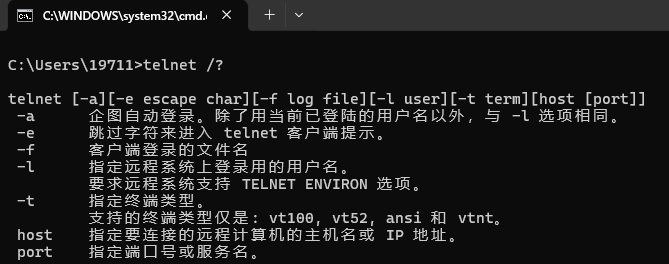
\includegraphics[width=0.7\textwidth]{figures/telnet.png}
  \caption{telnet /? 命令执行结果}
  \label{fig:jiwang}
\end{figure}

可以看到，我们可以指定远程服务器的 ip 和端口进行登录，也可以指定参数以实现自动登录。在登录后的终端页面，输入指定的 Escape 字符（默认为 Ctrl + ]），可以回退到 telnet 客户端界面。

进入 telnet 客户端页面，我们还可以查看针对管理页面的命令参数。

\begin{figure}[H]
  \centering
  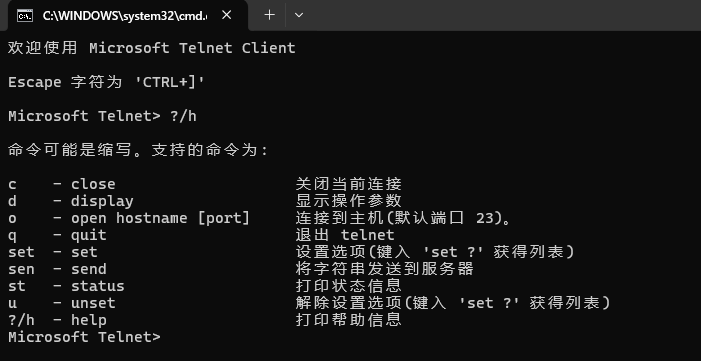
\includegraphics[width=0.65\textwidth]{figures/telnet_help.png}
  \caption{telnet 客户端帮助}
  \label{fig:jiwang}
\end{figure}

通过不同的指令，我们可以建立、关闭远程连接，向远程服务器发送字符串等。

\noindent {\heiti 应用与分析}

接下来，我们以虚拟机上的 ubuntu 服务器为例进行远程连接的测试。

通过查阅资料，先在 ubuntu 上开启了 telnet 服务端功能，并执行 ifconfig 来查看虚拟机的 ip地址。在本机客户端执行 telnet 192.168.35.128 之后，输入账号密码，就进入到了服务器的终端。

\begin{figure}[H]
  \centering
  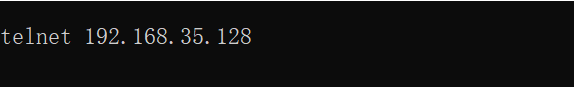
\includegraphics[width=0.6\textwidth]{figures/telnet_do.png}
  \caption{telnet 192.168.35.128}
  \label{fig:jiwang}
\end{figure}

\begin{figure}[H]
  \centering
  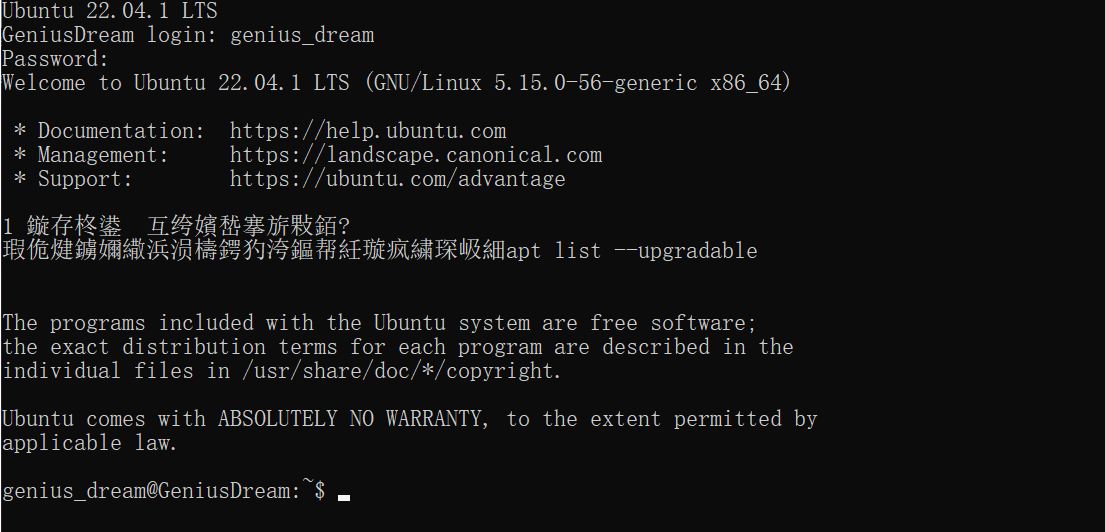
\includegraphics[width=0.7\textwidth]{figures/telnet_fwq.png}
  \caption{telnet 成功连接 ubuntu 服务器}
  \label{fig:jiwang}
\end{figure}

默认的 Escape 键是 Ctrl + ]，所以在上图的状态下按下输入 Ctrl + ]，我们就可以回到客户端进行其他操作。

在客户端我们执行 st 查看当前的连接状态，执行send hello 给服务器发送字符串”hello” ，运行结果如下图。

\begin{figure}[H]
  \centering
  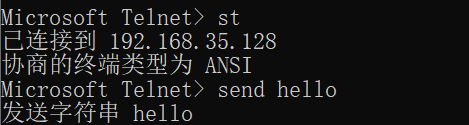
\includegraphics[width=0.6\textwidth]{figures/telnet_st.png}
  \caption{telnet 客户端操作示例及运行结果}
  \label{fig:jiwang}
\end{figure}

再次按下 Ctrl + V 和 Ctrl + M 可以回到远程终端环境。


% ---------- 2.2 交换机与路由器 ----------
\subsection{交换机与路由器}

\subsubsection{课程要求}

\begin{enumerate}[label=（\arabic*）, leftmargin=2em, itemsep=0.6em]
  \item 安装 Packet Tracer，在 Packet Tracer 仿真环境下，熟悉交换机命令与交换机初始化配置。
  \item 在交换机上实现 VLAN 配置；要求：创建三个 VLAN，给出拓扑，查看 VLAN 信息。
  \item 基于 Console 控制台登录配置路由器，学习路由器配置相关命令。
  \item 基于 Packet Tracer 构建网络环境，分别进行静态路由配置和基于 RIP 的动态路由配置；有余力的同学可设计基于 OSPF 的动态路由配置；能够进行综合集成网络情景设计更佳。
\end{enumerate}


\subsubsection{交换机命令学习及交换机初始化设置}

\noindent {\heiti 交换机的基本作用}

交换机是一种工作在数据链路层的网络设备，主要负责根据 MAC 地址表实现局域网内的数据转发。在本课程设计中，交换机主要用于构建局域网环境，为后续 VLAN 划分和跨 VLAN 通信实验提供基础平台。

\noindent {\heiti 交换机的必要性}

为保证实验环境的可控性与可重复性，在进行具体配置前，需要对交换机进行初始化设置，清除可能存在的历史配置，统一设备状态，避免旧配置对实验结果产生干扰。

\noindent {\heiti 交换机的初始化设置}

为完成后续 VLAN 划分及网络实验，需要首先对交换机进行初始化配置。以下列出了实验中常用的交换机基础命令及其功能说明。
\begin{enumerate}[label=（\arabic*）, leftmargin=2em, itemsep=1em]

  \item {\heiti 模式切换类命令}

  这些命令用于在不同配置层级之间切换，是所有配置操作的前提。

  \begin{itemize}
    \item \texttt{enable}：进入特权模式，用于查看和修改交换机配置。
    \item \texttt{configure terminal}：进入全局配置模式，对交换机进行整体配置。
    \item \texttt{interface <接口名>}：选择具体接口并进入端口配置模式，用于配置交换机端口属性。
    \item \texttt{exit}：退出当前配置模式，返回上一级模式。
    \item \texttt{end}：直接退出到特权模式，结束当前配置过程。
  \end{itemize}

  {\heiti 说明：}交换机配置具有层级结构，不同命令只能在对应模式下执行。

  \item {\heiti 交换机初始化常用命令}

  该类命令主要用于完成交换机的基础初始化配置，是后续实验的前提。

  \begin{itemize}
    \item \texttt{hostname <设备名>}：设置交换机名称，便于在多设备环境中区分不同交换机。
    \item \texttt{no ip domain-lookup}：关闭 DNS 查询功能，避免命令输入错误时系统长时间等待解析。
    \item \texttt{show running-config}：查看当前运行中的配置内容，用于检查初始化配置结果。
    \item \texttt{write} 或 \texttt{copy running-config startup-config}：保存当前配置，防止设备重启后配置丢失。
  \end{itemize}

  \item {\heiti VLAN 创建与管理命令}

  该类命令用于创建和管理 VLAN，为后续 VLAN 实验提供基础环境。

  \begin{itemize}
    \item \texttt{vlan <VLAN\_ID>}：创建并进入指定 VLAN 的配置模式。
    \item \texttt{name <VLAN 名称>}：为 VLAN 设置名称，提高配置的可读性。
    \item \texttt{show vlan} / \texttt{show vlan brief}：查看当前交换机上的 VLAN 信息及端口归属情况。
  \end{itemize}

  \item {\heiti 端口模式配置命令}

  该类命令用于配置交换机端口的工作模式及其 VLAN 属性。

  \begin{itemize}
    \item \texttt{switchport mode access}：将端口设置为 Access 模式，用于连接终端设备。
    \item \texttt{switchport access vlan <VLAN\_ID>}：指定端口所属的 VLAN。
    \item \texttt{switchport mode trunk}：将端口设置为 Trunk 模式，用于交换机之间或交换机与路由器之间传递多个 VLAN 数据。
  \end{itemize}

\end{enumerate}

通过上述初始化命令，对交换机的基本运行环境进行了统一设置，确保设备处于干净、稳定的状态，为后续 VLAN 划分及路由实验提供可靠的实验基础。

本部分通过对交换机常用命令的学习与初始化配置，掌握了交换机的基本操作流程和配置方法，为后续网络功能实验奠定了基础。

\subsubsection{交换机及 VLAN 配置}

\noindent {\heiti 网络拓扑结构与划分方案}

根据课程要求，我们在单交换机基础上构建三个VLAN进行试验，为了进一步进行交换机的知识学习，在原有课程要求的基础上，在跨交换机基础上也构建三个VLAN进行试验。

\begin{table}[H]
  \centering
  \caption{各主机 IP 地址的划分}
  \label{tab:host_ip}
  \begin{tabular}{cccc}
    \hline
    主机名称 & IP 地址 & 子网掩码 & 网关 \\ 
    \hline
    FPH51-PC0 & 192.168.10.2 & 255.255.255.0 & 缺省 \\ 
    FPH51-PC1 & 192.168.20.2 & 255.255.255.0 & 缺省 \\ 
    FPH51-PC2 & 192.168.30.2 & 255.255.255.0 & 缺省 \\ 
    FPH51-PC3 & 192.168.10.3 & 255.255.255.0 & 缺省 \\ 
    FPH51-PC4 & 192.168.20.3 & 255.255.255.0 & 缺省 \\ 
    FPH51-PC5 & 192.168.30.3 & 255.255.255.0 & 缺省 \\ 
    \hline
  \end{tabular}
\end{table}

(1) 单交换机
\begin{figure}[H]
  \centering
  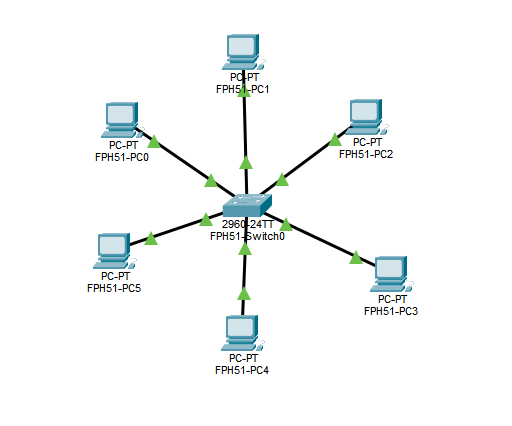
\includegraphics[width=0.7\textwidth]{figures/switch_dan.png}
  \caption{单交换机网络拓扑图}
  \label{fig:jiwang}
\end{figure}

(2) 跨交换机
\begin{figure}[H]
  \centering
  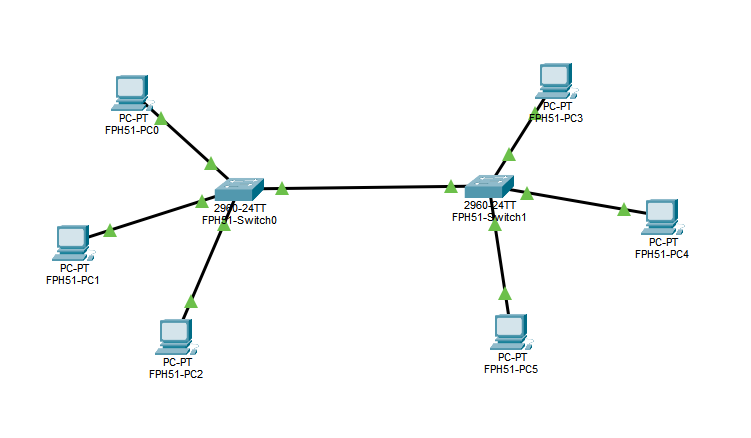
\includegraphics[width=0.7\textwidth]{figures/switch_kua.png}
  \caption{跨交换机网络拓扑图}
  \label{fig:jiwang}
\end{figure}

\noindent {\heiti 相关命令介绍}

\begin{itemize}
  \item \texttt{enable}：进入特权模式。
  \item \texttt{configure terminal}：进入全局配置模式。
  \item \texttt{interface}：选择一个接口进行配置，进入端口配置模式。
  \item \texttt{exit}：返回上一级。
  \item \texttt{end}：直接返回到特权模式。
  \item \texttt{vlan}：指定 VLAN ID，启用该 VLAN。
  \item \texttt{switchport access vlan}：在端口配置模式下，设置该端口对应的 VLAN。
  \item \texttt{switchport mode trunk}：在端口配置模式下，设置端口模式为 Trunk。
  \item \texttt{show vlan}：查看 VLAN 配置。
\end{itemize}

\noindent {\heiti 配置过程与结果分析}

由于交换机的配置都大小无异，我们这里只讲解单交换机情景下的配置过程，考虑到跨交换机配置雷同，为避免赘述，跨交换机情景只展示相关截图，不再重复文字赘述具体过程。

(1) 单交换机

单交换机配置过程如下，我们将 FPH51\_0 和 FPH51\_3 配置在 VLAN~10 下，
FPH51\_1 和 FPH51\_4 配置在 VLAN~20 下，
FPH51\_2 和 FPH51\_5 配置在 VLAN~30 下，具体命令操作如下：

\medskip

\begin{tabular}{p{6cm} p{8cm}}
\texttt{enable} & 进入特权模式 \\

\texttt{configure terminal} & 进入全局配置模式 \\

\texttt{vlan 10} & 创建并启用 VLAN~10 \\

\texttt{exit} & 退出 VLAN~10 配置模式 \\

\texttt{vlan 20} & 创建并启用 VLAN~20 \\

\texttt{exit} & 退出 VLAN~20 配置模式 \\

\texttt{vlan 30} & 创建并启用 VLAN~30 \\

\texttt{exit} & 退出 VLAN~30 配置模式 \\

\texttt{interface fastEthernet 0/1} & 进入端口 0/1 的配置模式 \\

\texttt{switchport mode access} & 将端口设置为 Access 模式 \\

\texttt{switchport access vlan 10} & 将端口 0/1 划分到 VLAN~10 \\

\texttt{exit} & 退出端口 0/1 配置模式 \\

\texttt{interface fastEthernet 0/2} & 进入端口 0/2 的配置模式 \\

\texttt{switchport mode access} & 将端口设置为 Access 模式 \\

\texttt{switchport access vlan 20} & 将端口 0/2 划分到 VLAN~20 \\

\texttt{exit} & 退出端口 0/2 配置模式 \\

\texttt{interface fastEthernet 0/3} & 进入端口 0/3 的配置模式 \\

\texttt{switchport mode access} & 将端口设置为 Access 模式 \\

\texttt{switchport access vlan 30} & 将端口 0/3 划分到 VLAN~30 \\

\texttt{exit} & 退出端口 0/3 配置模式 \\

\texttt{end} & 结束交换机配置，返回特权模式 \\

\texttt{show vlan} & 查看 VLAN 配置并验证端口划分情况 \\
\end{tabular}

为了简化操作，在Packet Tracer模拟环境下使用简化命令进行操作，详细简化命令如下表：

\begin{table}[H]
  \centering
  \caption{常用交换机命令及其简写形式}
  \label{tab:cmd_short}
  \begin{tabular}{llll}
    \hline
    命令全称 & 常用简写 & 命令全称 & 常用简写 \\
    \hline
    \texttt{enable} & \texttt{en} &
    \texttt{configure terminal} & \texttt{conf t} \\

    \texttt{interface} & \texttt{int} &
    \texttt{interface range} & \texttt{int ra} \\

    \texttt{switchport mode access} & \texttt{sw mo acc} &
    \texttt{switchport access vlan} & \texttt{sw acc vlan} \\

    \texttt{show vlan} & \texttt{sh vlan} &
    \texttt{show vlan brief} & \texttt{sh vlan br} \\

    \texttt{exit} & \texttt{ex} &
    &  \\
    \hline
  \end{tabular}
\end{table}

\begin{figure}[H]
  \centering
  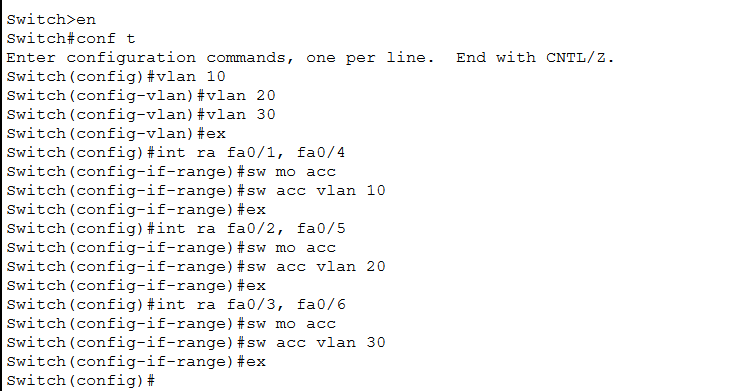
\includegraphics[width=0.65\textwidth]{figures/switch_dan_peizhi.png}
  \caption{单交换机 VLAN 配置过程}
  \label{fig:jiwang}
\end{figure}

配置结束后，使用 show vlan 查看该交换机的配置情况，结果符合预期。

\begin{figure}[H]
  \centering
  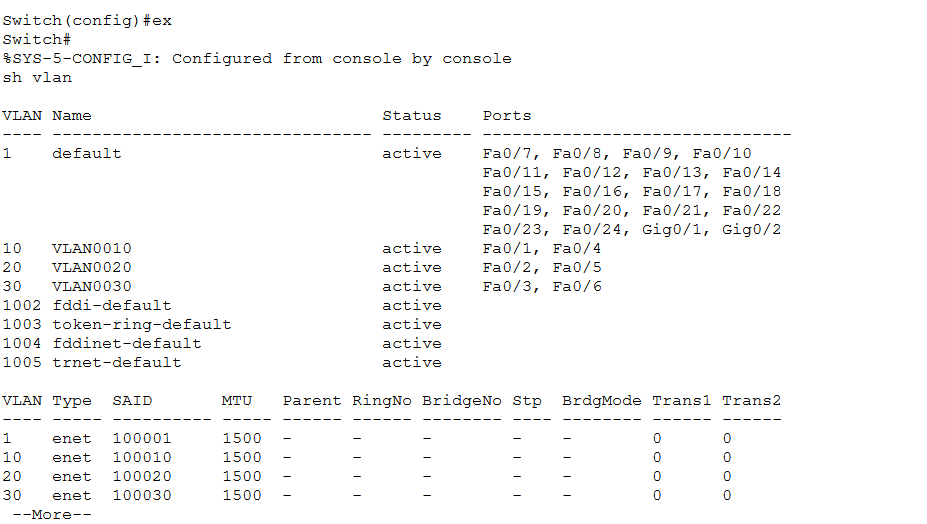
\includegraphics[width=0.65\textwidth]{figures/switch_dan_show.png}
  \caption{单交换机 VLAN 配置过程}
  \label{fig:jiwang}
\end{figure}

(2) 跨交换机
配置 Trunk 端口后，同一 VLAN 内的主机可实现跨交换机通信，跨交换机配置过程如下（两交换机一致，仅展示FPH51\_Switch0）：

\begin{figure}[H]
  \centering
  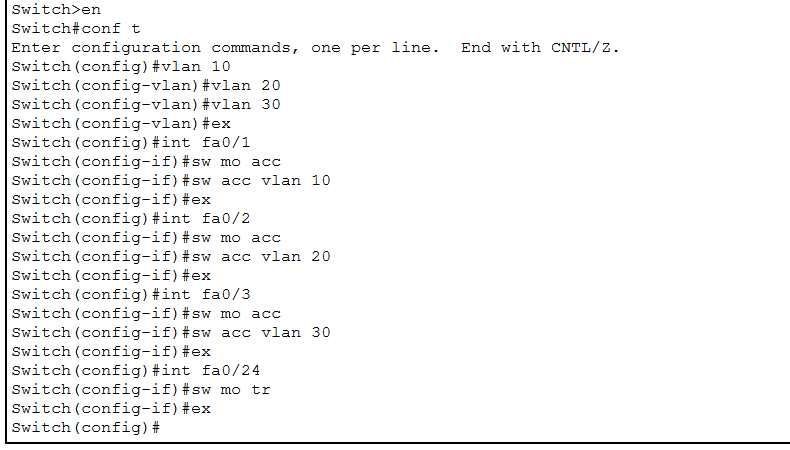
\includegraphics[width=0.6\textwidth]{figures/switch_kua_sw1.png}
  \caption{跨交换机 Switch0 配置过程}
  \label{fig:jiwang}
\end{figure}

配置结果如下图：

\begin{figure}[H]
  \centering
  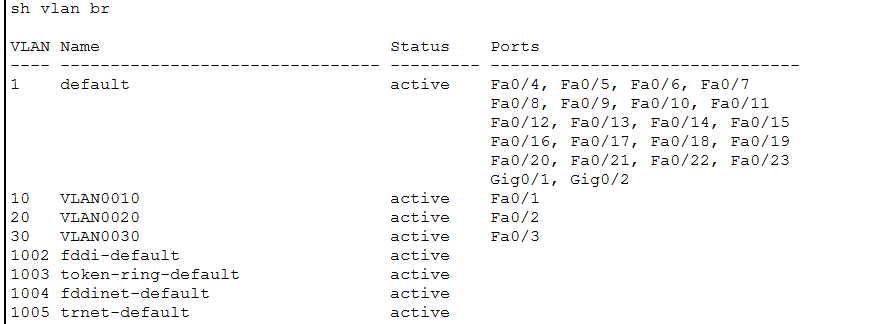
\includegraphics[width=0.8\textwidth]{figures/switch_kua_show.png}
  \caption{跨交换机 VLAN 配置完成后检查配置文件}
  \label{fig:jiwang}
\end{figure}

PC0分别 ping 同一 VLAN 下的 PC3(192.168.10.3)和不同 VLAN 下的 PC1 (192.168 .20. 2)， 发现交换机两端同一 VLAN 的主机可以相互 ping 通，不同 VLAN 的主机 ping 不通，如下图:

\begin{figure}[H]
  \centering
  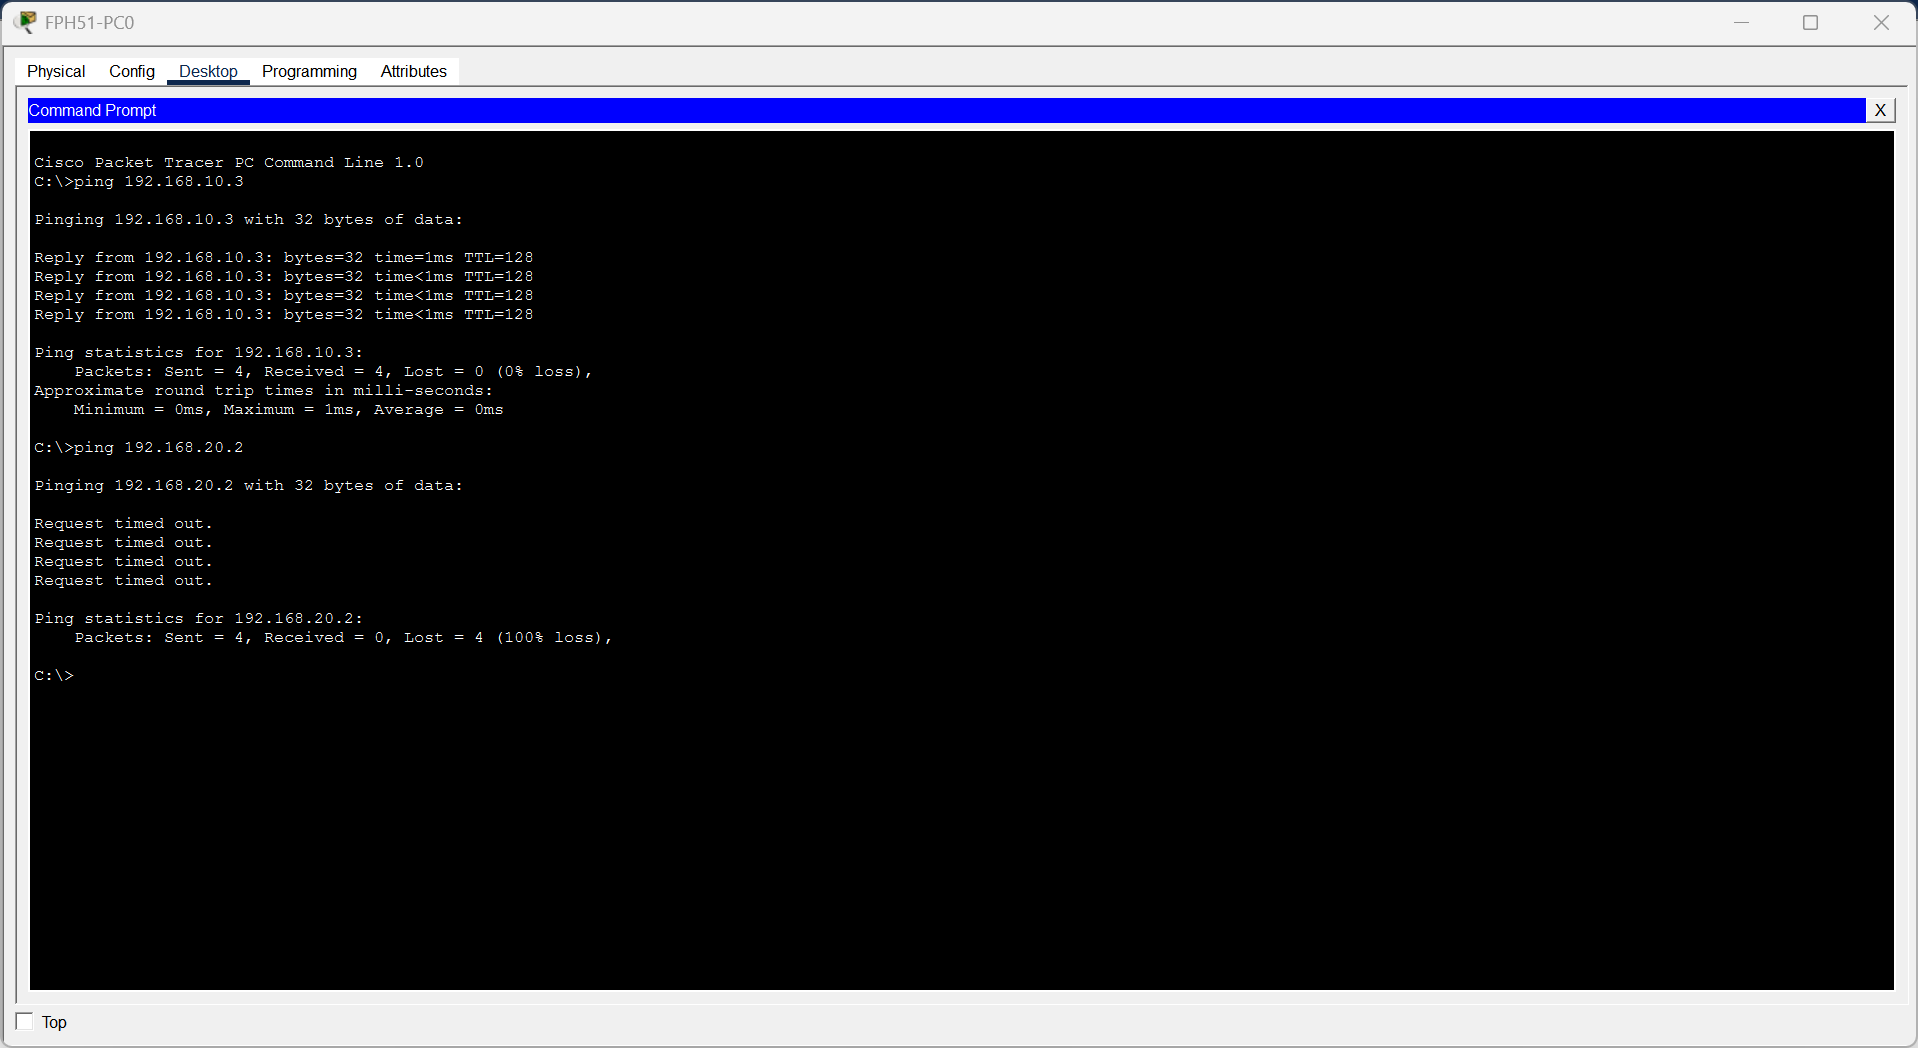
\includegraphics[width=1.0\textwidth]{figures/02_PC0_ping.png}
  \caption{主机 FPH51\_PC0 ping 同一 VLAN 和不同 VLAN 下的主机}
  \label{fig:jiwang}
\end{figure}

\subsubsection{路由器命令学习及路由器初始化设置}

\noindent {\heiti 路由器的基本作用}

路由器是一种工作在网络层的网络设备，主要用于根据路由表实现不同网络之间的数据转发。在本课程设计中，路由器用于连接不同网段，实现跨网段通信以及静态路由和动态路由协议的配置，是构建复杂网络拓扑的重要组成部分。

\noindent {\heiti 路由器配置的必要性}

在进行路由实验前，需要对路由器进行基础配置和初始化设置，以确保设备处于可控、稳定的工作状态。通过规范的初始化操作，可以避免历史配置对实验结果的干扰，并为后续路由协议配置提供统一的实验环境。

\noindent {\heiti 路由器的初始化设置}

为完成后续静态路由及动态路由实验，需要首先对路由器进行初始化配置。以下列出了实验中常用的路由器基础命令及其功能说明。

\begin{enumerate}[label=（\arabic*）, leftmargin=2em, itemsep=1em]

  \item {\heiti 模式切换类命令}

  该类命令用于在不同配置层级之间切换，是路由器配置操作的基础。

  \begin{itemize}
    \item \texttt{enable}：进入特权模式，用于查看路由器状态及进行高级配置。
    \item \texttt{configure terminal}：进入全局配置模式，对路由器进行整体参数设置。
    \item \texttt{interface <接口名>}：进入指定接口的配置模式，用于配置接口的 IP 地址及状态。
    \item \texttt{exit}：退出当前配置模式，返回上一级模式。
    \item \texttt{end}：直接返回特权模式，结束当前配置过程。
  \end{itemize}

  {\heiti 说明：}路由器配置同样采用分层结构，不同类型的命令只能在对应的配置模式下执行。

  \item {\heiti 路由器初始化常用命令}

  该类命令主要用于完成路由器的基础初始化设置，为后续路由功能配置提供前提条件。

  \begin{itemize}
    \item \texttt{hostname <设备名>}：设置路由器名称，便于在多路由器环境中区分不同设备。
    \item \texttt{no ip domain-lookup}：关闭 DNS 查询功能，避免因误输入命令导致系统长时间等待解析。
    \item \texttt{show running-config}：查看当前运行配置，用于检查初始化配置是否正确。
    \item \texttt{write} 或 \texttt{copy running-config startup-config}：保存当前配置，防止设备重启后配置丢失。
  \end{itemize}

  \item {\heiti 接口配置相关命令}

  该类命令用于配置路由器接口的 IP 参数及接口状态，是实现网络互联的基础。

  \begin{itemize}
    \item \texttt{interface g0/0} / \texttt{interface f0/0}：进入指定物理接口的配置模式。
    \item \texttt{ip add <IP地址> <子网掩码>}：为接口配置 IP 地址及子网掩码。
    \item \texttt{no shutdown}：启用接口，使接口由关闭状态变为工作状态。
  \end{itemize}

  \item {\heiti 路由查看与验证命令}

  该类命令用于查看路由器当前的接口状态和路由信息，是验证配置结果的重要手段。

  \begin{itemize}
    \item \texttt{show ip interface brief}：查看各接口的 IP 地址及接口状态。
    \item \texttt{show ip route}：查看路由器的路由表信息，用于验证路由配置是否生效。
    \item \texttt{show running-config}：检查当前路由器的整体配置情况。
  \end{itemize}

\end{enumerate}

通过上述路由器初始化配置命令，对路由器的基本运行环境和接口参数进行了统一设置，为后续静态路由和动态路由协议的配置提供了可靠的基础条件。

本部分通过对路由器常用命令及登录配置方法的学习，掌握了路由器的基本操作流程和初始化配置方法，为后续路由功能实验的顺利开展奠定了基础。


\subsubsection{静态路由配置}

\noindent {\heiti 网络拓扑结构与划分方案}

根据课程要求，我们进行静态路由的配置。

网络拓扑结构如下图：

\begin{figure}[H]
  \centering
  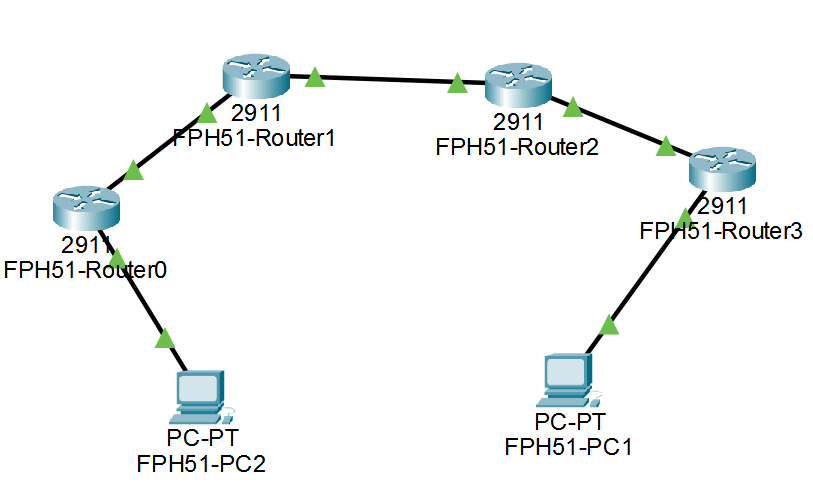
\includegraphics[width=0.7\textwidth]{figures/jingtai.png}
  \caption{静态路由配置拓扑图}
  \label{fig:jiwang}
\end{figure}

网络划分方案如下：

\begin{table}[H]
\centering
\caption{静态路由实验网络地址规划表}
\begin{tabular}{ccccc}
\hline
设备名称 & 接口名称 & IP 地址 & 子网掩码 & 默认网关 \\
\hline
FPH51\_PC1 & FastEthernet0 & 192.168.4.2 & 255.255.255.0 & 192.168.4.1 \\
FPH51\_PC2 & FastEthernet0 & 192.168.1.2 & 255.255.255.0 & 192.168.1.1 \\
FPH51\_Router0 & GigabitEthernet0/0 & 192.168.1.1 & 255.255.255.0 & — \\
FPH51\_Router0 & GigabitEthernet0/1 & 10.0.12.1 & 255.255.255.0 & — \\
FPH51\_Router1 & GigabitEthernet0/0 & 10.0.12.2 & 255.255.255.0 & — \\
FPH51\_Router1 & GigabitEthernet0/1 & 10.0.23.1 & 255.255.255.0 & — \\
FPH51\_Router2 & GigabitEthernet0/0 & 10.0.23.2 & 255.255.255.0 & — \\
FPH51\_Router2 & GigabitEthernet0/1 & 10.0.34.1 & 255.255.255.0 & — \\
FPH51\_Router3 & GigabitEthernet0/0 & 10.0.34.2 & 255.255.255.0 & — \\
FPH51\_Router3 & GigabitEthernet0/1 & 192.168.4.1 & 255.255.255.0 & — \\
\hline
\end{tabular}
\end{table}

\subsubsection*{相关命令介绍}

\begin{itemize}
  \item \texttt{enable}：进入特权模式。
  \item \texttt{configure terminal}：进入全局配置模式。
  \item \texttt{interface}：选择一个接口进行配置，进入端口配置模式。
  \item \texttt{line}：指定参数后进入行配置模式。
  \item \texttt{exit}：返回上一级模式。
  \item \texttt{end}：直接返回到特权模式。
  \item \texttt{show ip route}：查看路由器的路由表项。
  \item \texttt{ip route add NETMASK NEXTHOP}：更新路由表项。
\end{itemize}

\noindent {\heiti 配置过程与结果分析}

通过依次配置这四个路由，我们将使得 FPH51\_PC1 与 FPH51\_PC2 能够相互通信。

\noindent\textbf{配置路由 FPH51\_Router0：}

\medskip

\begin{tabular}{p{7cm} p{7cm}}
\texttt{enable} & 进入特权模式 \\

\texttt{configure terminal} & 进入全局配置模式 \\

\texttt{ip route 192.168.4.0 255.255.255.0 10.0.23.1}
& 配置到 192.168.4.0/24 网络的静态路由 \\

\texttt{exit} & 退出全局配置模式 \\

\texttt{show ip route} & 查看并验证静态路由配置结果 \\
\end{tabular}

\noindent\textbf{配置路由 FPH51\_Router1：}

\medskip

\begin{tabular}{p{7cm} p{7cm}}
\texttt{enable} & 进入特权模式 \\
\texttt{configure terminal} & 进入全局配置模式 \\

\texttt{ip route 192.168.1.0 255.255.255.0 10.0.23.2}
& 配置到 192.168.1.0/24 网络的静态路由 \\

\texttt{ip route 192.168.4.0 255.255.255.0 10.0.23.2}
& 配置到 192.168.4.0/24 网络的静态路由 \\

\texttt{exit} & 退出全局配置模式 \\
\texttt{show ip route} & 查看并验证静态路由配置结果 \\
\end{tabular}

\noindent\textbf{配置路由 FPH51\_Router2：}

\medskip

\begin{tabular}{p{7cm} p{7cm}}
\texttt{enable} & 进入特权模式 \\
\texttt{configure terminal} & 进入全局配置模式 \\

\texttt{ip route 192.168.4.0 255.255.255.0 10.0.23.1}
& 配置到 192.168.4.0/24 网络的静态路由 \\

\texttt{exit} & 退出全局配置模式 \\
\texttt{show ip route} & 查看并验证静态路由配置结果 \\
\end{tabular}

\noindent\textbf{配置路由 FPH51\_Router3：}

\medskip

\begin{tabular}{p{7cm} p{7cm}}
\texttt{enable} & 进入特权模式 \\
\texttt{configure terminal} & 进入全局配置模式 \\

\texttt{ip route 192.168.1.0 255.255.255.0 192.168.4.2}
& 配置到 192.168.1.0/24 网络的静态路由 \\

\texttt{exit} & 退出全局配置模式 \\
\texttt{show ip route} & 查看并验证静态路由配置结果 \\
\end{tabular}


配置完成后，我们可以使用 show ip route 查看各路由器的路由表以验证是否配置成功。以 FPH51\_Router0 为例，其路由表如下：

\begin{figure}[H]
  \centering
  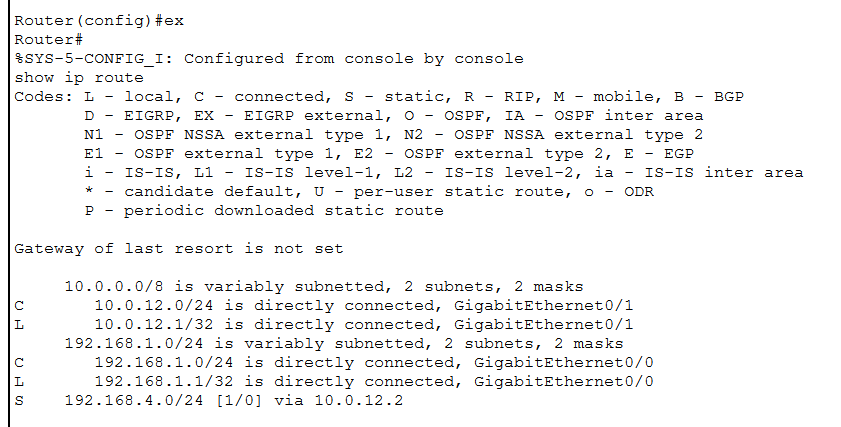
\includegraphics[width=0.7\textwidth]{figures/jingtai_show.png}
  \caption{FPH51\_Router0 的路由表}
  \label{fig:jiwang}
\end{figure}

静态路由配置成功后，我们使用 ping 命令来验证 FPH51\_PC1 和 FPH51\_PC2 的可达性，结果符合我们的预期。

\begin{figure}[H]
  \centering
  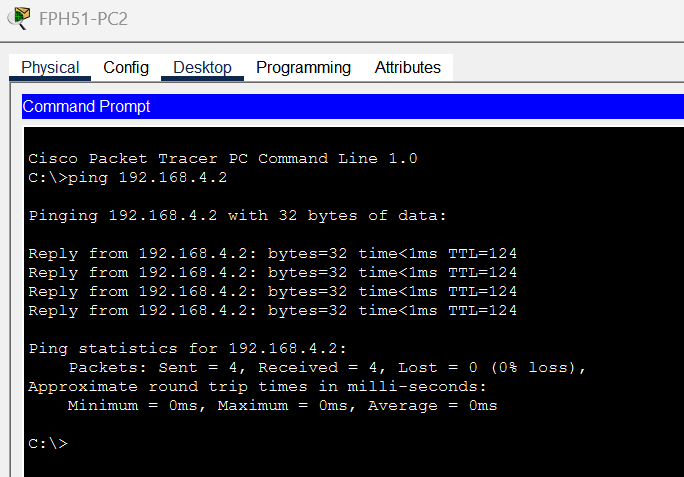
\includegraphics[width=0.8\textwidth]{figures/jingtai_ping.png}
  \caption{静态路由配置结果验证}
  \label{fig:jiwang}
\end{figure}


\subsubsection{动态路由配置 RIP}

\noindent {\heiti 网络拓扑结构与划分方案}

根据课程要求，我们使用 RIP 配置动态路由。

如图所示，我们构造了以下网络拓扑结构:

\begin{figure}[H]
  \centering
  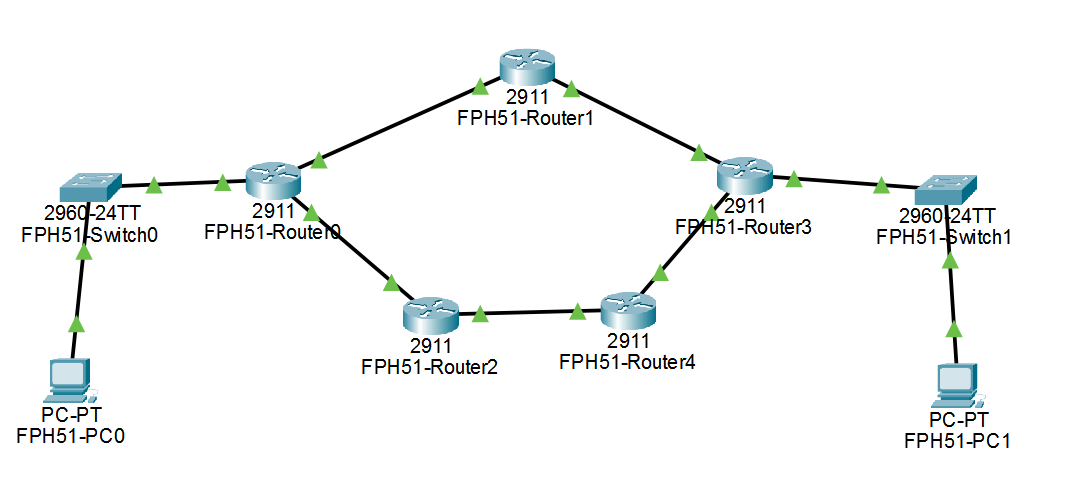
\includegraphics[width=0.7\textwidth]{figures/RIP.png}
  \caption{RIP 动态路由配置拓扑结构图}
  \label{fig:jiwang}
\end{figure}

\begin{table}[H]
\centering
\caption{静态路由实验网络地址规划表}
\begin{tabular}{ccccc}
\hline
设备名称 & 接口名称 & IP 地址 & 子网掩码 & 默认网关 \\
\hline
FPH51\_PC0 & FastEthernet0 & 192.168.1.2 & 255.255.255.0 & 192.168.1.1 \\
FPH51\_PC1 & FastEthernet0 & 192.168.4.2 & 255.255.255.0 & 192.168.4.1 \\
FPH51\_Router0 & GigabitEthernet0/0 & 192.168.1.1 & 255.255.255.0 & — \\
FPH51\_Router0 & GigabitEthernet0/1 & 10.0.12.1 & 255.255.255.0 & — \\
FPH51\_Router0 & GigabitEthernet0/2 & 10.0.13.1 & 255.255.255.0 & — \\
FPH51\_Router1 & GigabitEthernet0/0 & 10.0.12.2 & 255.255.255.0 & — \\
FPH51\_Router1 & GigabitEthernet0/1 & 10.0.24.1 & 255.255.255.0 & — \\
FPH51\_Router2 & GigabitEthernet0/0 & 10.0.13.2 & 255.255.255.0 & — \\
FPH51\_Router2 & GigabitEthernet0/1 & 10.0.35.1 & 255.255.255.0 & — \\
FPH51\_Router3 & GigabitEthernet0/0 & 10.0.24.2 & 255.255.255.0 & — \\
FPH51\_Router3 & GigabitEthernet0/1 & 10.0.54.2 & 255.255.255.0 & — \\
FPH51\_Router3 & GigabitEthernet0/2 & 192.168.4.1 & 255.255.255.0 & — \\
FPH51\_Router4 & GigabitEthernet0/0 & 10.0.35.2 & 255.255.255.0 & — \\
FPH51\_Router4 & GigabitEthernet0/1 & 10.0.54.1 & 255.255.255.0 & — \\
\hline
\end{tabular}
\end{table}

\subsubsection*{相关命令介绍}

\begin{itemize}
  \item \texttt{show ip route}：查看路由器的路由表项。
  \item \texttt{router rip}：进入 RIP 动态路由配置模式。
  \item \texttt{net IP}：在 RIP 配置模式下设置邻接设备地址。
  \item \texttt{version VERSION}：在 RIP 配置模式下设置 RIP 版本。
  \item \texttt{ip routing}：开启路由功能。
\end{itemize}

\noindent {\heiti 配置过程与结果分析}

通过依次配置这五个路由为 RIP 动态路由后，我们将使得 FPH51\_PC0 与 FPH51\_PC1 能够相互通信。不同于静态路由的是，他们之间进行通信时，传输的 IP 报将选择最少跳的路线到达目的地址。

%================================================
% FPH51_R0
%================================================
\noindent\textbf{配置路由 FPH51\_Router0：}

\medskip
\begin{tabular}{p{7cm} p{7cm}}
\texttt{enable} & 进入特权模式 \\
\texttt{configure terminal} & 进入全局配置模式 \\

\texttt{interface g0/0} & 进入接口 g0/0 配置模式 \\
\texttt{ip add 192.168.1.1 255.255.255.0} & 配置接口 IP 地址 \\
\texttt{no shutdown} & 启用接口 \\
\texttt{exit} & 退出接口配置模式 \\

\texttt{interface g0/1} & 进入接口 g0/1 配置模式 \\
\texttt{ip add 10.0.12.1 255.255.255.0} & 配置接口 IP 地址 \\
\texttt{no shutdown} & 启用接口 \\
\texttt{exit} & 退出接口配置模式 \\

\texttt{interface g0/2} & 进入接口 g0/2 配置模式 \\
\texttt{ip add 10.0.13.1 255.255.255.0} & 配置接口 IP 地址 \\
\texttt{no shutdown} & 启用接口 \\

\texttt{end} & 返回特权模式 \\
\end{tabular}

\bigskip
\begin{tabular}{p{7cm} p{7cm}}
\texttt{configure terminal} & 进入全局配置模式 \\
\texttt{router rip} & 进入 RIP 配置模式 \\
\texttt{version 2} & 设置 RIP 版本为 v2 \\
\texttt{no auto-summary} & 关闭自动汇总 \\
\texttt{net 192.168.1.0} & 宣告直连网络 \\
\texttt{net 10.0.12.0} & 宣告直连网络 \\
\texttt{net 10.0.13.0} & 宣告直连网络 \\
\texttt{end} & 返回特权模式 \\
\end{tabular}

%================================================
% FPH51_R1
%================================================
\bigskip
\noindent\textbf{配置路由 FPH51\_Router1：}

\medskip
\begin{tabular}{p{7cm} p{7cm}}
\texttt{enable} & 进入特权模式 \\
\texttt{configure terminal} & 进入全局配置模式 \\

\texttt{interface g0/0} & 进入接口 g0/0 配置模式 \\
\texttt{ip add 10.0.12.2 255.255.255.0} & 配置接口 IP 地址 \\
\texttt{no shutdown} & 启用接口 \\
\texttt{exit} & 退出接口配置模式 \\

\texttt{interface g0/1} & 进入接口 g0/1 配置模式 \\
\texttt{ip add 10.0.24.1 255.255.255.0} & 配置接口 IP 地址 \\
\texttt{no shutdown} & 启用接口 \\

\texttt{end} & 返回特权模式 \\
\end{tabular}

\bigskip
\begin{tabular}{p{7cm} p{7cm}}
\texttt{configure terminal} & 进入全局配置模式 \\
\texttt{router rip} & 进入 RIP 配置模式 \\
\texttt{version 2} & 设置 RIP 版本为 v2 \\
\texttt{no auto-summary} & 关闭自动汇总 \\
\texttt{net 10.0.12.0} & 宣告直连网络 \\
\texttt{net 10.0.24.0} & 宣告直连网络 \\
\texttt{end} & 返回特权模式 \\
\end{tabular}

%================================================
% FPH51_R2
%================================================
\bigskip
\noindent\textbf{配置路由 FPH51\_Router2：}

\medskip
\begin{tabular}{p{7cm} p{7cm}}
\texttt{enable} & 进入特权模式 \\
\texttt{configure terminal} & 进入全局配置模式 \\

\texttt{interface g0/0} & 进入接口 g0/0 配置模式 \\
\texttt{ip add 10.0.13.2 255.255.255.0} & 配置接口 IP 地址 \\
\texttt{no shutdown} & 启用接口 \\
\texttt{exit} & 退出接口配置模式 \\

\texttt{interface g0/1} & 进入接口 g0/1 配置模式 \\
\texttt{ip add 10.0.35.1 255.255.255.0} & 配置接口 IP 地址 \\
\texttt{no shutdown} & 启用接口 \\

\texttt{end} & 返回特权模式 \\
\end{tabular}

\bigskip
\begin{tabular}{p{7cm} p{7cm}}
\texttt{configure terminal} & 进入全局配置模式 \\
\texttt{router rip} & 进入 RIP 配置模式 \\
\texttt{version 2} & 设置 RIP 版本为 v2 \\
\texttt{no auto-summary} & 关闭自动汇总 \\
\texttt{net 10.0.13.0} & 宣告直连网络 \\
\texttt{net 10.0.35.0} & 宣告直连网络 \\
\texttt{end} & 返回特权模式 \\
\end{tabular}

%================================================
% FPH51_R3
%================================================
\bigskip
\noindent\textbf{配置路由 FPH51\_Router3：}

\medskip
\begin{tabular}{p{7cm} p{7cm}}
\texttt{enable} & 进入特权模式 \\
\texttt{configure terminal} & 进入全局配置模式 \\

\texttt{interface g0/0} & 进入接口 g0/0 配置模式 \\
\texttt{ip add 10.0.35.2 255.255.255.0} & 配置接口 IP 地址 \\
\texttt{no shutdown} & 启用接口 \\
\texttt{exit} & 退出接口配置模式 \\

\texttt{interface g0/1} & 进入接口 g0/1 配置模式 \\
\texttt{ip add 10.0.54.1 255.255.255.0} & 配置接口 IP 地址 \\
\texttt{no shutdown} & 启用接口 \\

\texttt{end} & 返回特权模式 \\
\end{tabular}

\bigskip
\begin{tabular}{p{7cm} p{7cm}}
\texttt{configure terminal} & 进入全局配置模式 \\
\texttt{router rip} & 进入 RIP 配置模式 \\
\texttt{version 2} & 设置 RIP 版本为 v2 \\
\texttt{no auto-summary} & 关闭自动汇总 \\
\texttt{net 10.0.35.0} & 宣告直连网络 \\
\texttt{net 10.0.54.0} & 宣告直连网络 \\
\texttt{end} & 返回特权模式 \\
\end{tabular}

%================================================
% FPH51_R4
%================================================
\bigskip
\noindent\textbf{配置路由 FPH51\_Router4：}

\medskip
\begin{tabular}{p{7cm} p{7cm}}
\texttt{enable} & 进入特权模式 \\
\texttt{configure terminal} & 进入全局配置模式 \\

\texttt{interface g0/0} & 进入接口 g0/0 配置模式 \\
\texttt{ip add 10.0.24.2 255.255.255.0} & 配置接口 IP 地址 \\
\texttt{no shutdown} & 启用接口 \\
\texttt{exit} & 退出接口配置模式 \\

\texttt{interface g0/1} & 进入接口 g0/1 配置模式 \\
\texttt{ip add 10.0.54.2 255.255.255.0} & 配置接口 IP 地址 \\
\texttt{no shutdown} & 启用接口 \\
\texttt{exit} & 退出接口配置模式 \\

\texttt{interface g0/2} & 进入接口 g0/2 配置模式 \\
\texttt{ip add 192.168.4.1 255.255.255.0} & 配置接口 IP 地址 \\
\texttt{no shutdown} & 启用接口 \\

\texttt{end} & 返回特权模式 \\
\end{tabular}

\bigskip
\begin{tabular}{p{7cm} p{7cm}}
\texttt{configure terminal} & 进入全局配置模式 \\
\texttt{router rip} & 进入 RIP 配置模式 \\
\texttt{version 2} & 设置 RIP 版本为 v2 \\
\texttt{no auto-summary} & 关闭自动汇总 \\
\texttt{net 10.0.24.0} & 宣告直连网络 \\
\texttt{net 10.0.54.0} & 宣告直连网络 \\
\texttt{net 192.168.4.0} & 宣告直连网络 \\
\texttt{end} & 返回特权模式 \\
\end{tabular}

\vspace{1em}
然后将所有路由器都开启RIP：

\noindent\textbf{开启 RIP 的路由 FPH51\_Router0：}

\medskip
\begin{tabular}{p{7cm} p{7cm}}
\texttt{configure terminal} & 进入全局配置模式 \\
\texttt{router rip} & 进入 RIP 动态路由配置模式 \\
\texttt{version 2} & 设置 RIP 版本为 v2 \\
\texttt{no auto-summary} & 关闭自动汇总功能 \\
\texttt{net 192.168.1.0} & 宣告直连网络 192.168.1.0/24 \\
\texttt{net 10.0.12.0} & 宣告直连网络 10.0.12.0/24 \\
\texttt{net 10.0.13.0} & 宣告直连网络 10.0.13.0/24 \\
\texttt{end} & 返回特权模式 \\
\end{tabular}

\bigskip
\noindent\textbf{开启 RIP 的路由 FPH51\_Router1：}

\medskip
\begin{tabular}{p{7cm} p{7cm}}
\texttt{configure terminal} & 进入全局配置模式 \\
\texttt{router rip} & 进入 RIP 动态路由配置模式 \\
\texttt{version 2} & 设置 RIP 版本为 v2 \\
\texttt{no auto-summary} & 关闭自动汇总功能 \\
\texttt{net 10.0.12.0} & 宣告直连网络 10.0.12.0/24 \\
\texttt{net 10.0.24.0} & 宣告直连网络 10.0.24.0/24 \\
\texttt{end} & 返回特权模式 \\
\end{tabular}

\bigskip
\noindent\textbf{开启 RIP 的路由 FPH51\_Router2：}

\medskip
\begin{tabular}{p{7cm} p{7cm}}
\texttt{configure terminal} & 进入全局配置模式 \\
\texttt{router rip} & 进入 RIP 动态路由配置模式 \\
\texttt{version 2} & 设置 RIP 版本为 v2 \\
\texttt{no auto-summary} & 关闭自动汇总功能 \\
\texttt{net 10.0.13.0} & 宣告直连网络 10.0.13.0/24 \\
\texttt{net 10.0.35.0} & 宣告直连网络 10.0.35.0/24 \\
\texttt{end} & 返回特权模式 \\
\end{tabular}

\bigskip
\noindent\textbf{开启 RIP 的路由 FPH51\_Router3：}

\medskip
\begin{tabular}{p{7cm} p{7cm}}
\texttt{configure terminal} & 进入全局配置模式 \\
\texttt{router rip} & 进入 RIP 动态路由配置模式 \\
\texttt{version 2} & 设置 RIP 版本为 v2 \\
\texttt{no auto-summary} & 关闭自动汇总功能 \\
\texttt{net 10.0.35.0} & 宣告直连网络 10.0.35.0/24 \\
\texttt{net 10.0.54.0} & 宣告直连网络 10.0.54.0/24 \\
\texttt{end} & 返回特权模式 \\
\end{tabular}

\bigskip
\noindent\textbf{开启 RIP 的路由 FPH51\_Router4：}

\medskip
\begin{tabular}{p{7cm} p{7cm}}
\texttt{configure terminal} & 进入全局配置模式 \\
\texttt{router rip} & 进入 RIP 动态路由配置模式 \\
\texttt{version 2} & 设置 RIP 版本为 v2 \\
\texttt{no auto-summary} & 关闭自动汇总功能 \\
\texttt{net 10.0.24.0} & 宣告直连网络 10.0.24.0/24 \\
\texttt{net 10.0.54.0} & 宣告直连网络 10.0.54.0/24 \\
\texttt{net 192.168.4.0} & 宣告直连网络 192.168.4.0/24 \\
\texttt{end} & 返回特权模式 \\
\end{tabular}

当配置完所有设备后，我们可以使用 show ip route 来检验路由配置结果。以交换机 FPH51\_Router0 为例，配置结果如下图所示：

\begin{figure}[H]
  \centering
  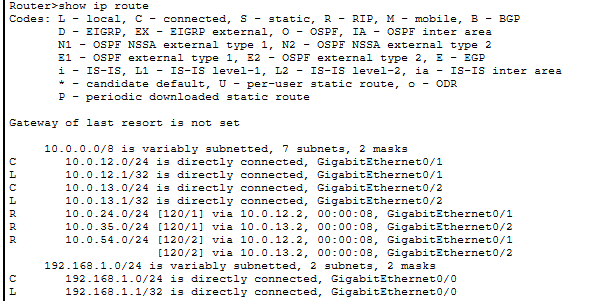
\includegraphics[width=0.7\textwidth]{figures/RIP_show.png}
  \caption{RIP 路由配置后的路由表}
  \label{fig:jiwang}
\end{figure}

我们可以看到，这个路由表是符合预期的。

\begin{figure}[H]
  \centering
  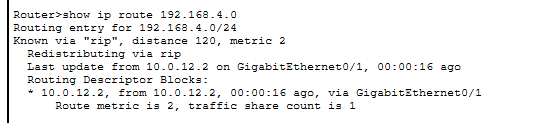
\includegraphics[width=0.7\textwidth]{figures/RIP_show_least.png}
  \caption{RIP 路径选择}
  \label{fig:jiwang}
\end{figure}

可以看到，FPH51\_Router0到\ 192.168.4.0\ 的RIP路由走的是\ 10.0.12.2\ ，即FPH51\_Router1这一条路径，因为这条路径跳数最短，为最短路，所以RIP动态路由下选择这条路

\begin{figure}[H]
  \centering
  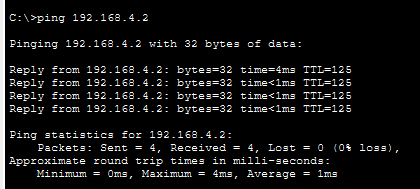
\includegraphics[width=0.7\textwidth]{figures/RIP_ping.png}
  \caption{RIP动态路由验证截图}
  \label{fig:jiwang}
\end{figure}

发现FPH51\_PC0和FPH51\_PC1可以\ ping\ 的通，说明成功实现了RIP动态路由并且两台PC联通。

\subsubsection{动态路由配置 OSPF}

OSPF动态路由可以在前面已有的RIP动态路由基础上修改实现，这里简略介绍，不再进行赘述，进介绍基础操作过程：

在所有路由器上执行以下操作，关闭 RIP 动态路由协议：

\medskip
\begin{tabular}{p{7cm} p{7cm}}
\texttt{configure terminal} & 进入全局配置模式 \\
\texttt{no router rip} & 关闭 RIP 动态路由协议 \\
\texttt{end} & 返回特权模式 \\
\end{tabular}

\noindent\textbf{开启 OSPF 的路由 FPH51\_R0：}

\medskip
\begin{tabular}{p{7cm} p{7cm}}
\texttt{configure terminal} & 进入全局配置模式 \\
\texttt{router ospf 1} & 创建并进入 OSPF 进程 1 \\
\texttt{net 192.168.1.0 0.0.0.255 area 0} & 宣告直连网络加入 Area~0 \\
\texttt{net 10.0.12.0 0.0.0.255 area 0} & 宣告直连网络加入 Area~0 \\
\texttt{net 10.0.13.0 0.0.0.255 area 0} & 宣告直连网络加入 Area~0 \\
\texttt{end} & 返回特权模式 \\
\end{tabular}

\bigskip
\noindent\textbf{开启 OSPF 的路由 FPH51\_R1：}

\medskip
\begin{tabular}{p{7cm} p{7cm}}
\texttt{configure terminal} & 进入全局配置模式 \\
\texttt{router ospf 1} & 创建并进入 OSPF 进程 1 \\
\texttt{net 10.0.12.0 0.0.0.255 area 0} & 宣告直连网络加入 Area~0 \\
\texttt{net 10.0.24.0 0.0.0.255 area 0} & 宣告直连网络加入 Area~0 \\
\texttt{end} & 返回特权模式 \\
\end{tabular}



\bigskip
\noindent\textbf{开启 OSPF 的路由 FPH51\_R2：}

\medskip
\begin{tabular}{p{7cm} p{7cm}}
\texttt{configure terminal} & 进入全局配置模式 \\
\texttt{router ospf 1} & 创建并进入 OSPF 进程 1 \\
\texttt{net 10.0.13.0 0.0.0.255 area 0} & 宣告直连网络加入 Area~0 \\
\texttt{net 10.0.35.0 0.0.0.255 area 0} & 宣告直连网络加入 Area~0 \\
\texttt{end} & 返回特权模式 \\
\end{tabular}

\bigskip
\noindent\textbf{开启 OSPF 的路由 FPH51\_R3：}

\medskip
\begin{tabular}{p{7cm} p{7cm}}
\texttt{configure terminal} & 进入全局配置模式 \\
\texttt{router ospf 1} & 创建并进入 OSPF 进程 1 \\
\texttt{net 10.0.35.0 0.0.0.255 area 0} & 宣告直连网络加入 Area~0 \\
\texttt{net 10.0.54.0 0.0.0.255 area 0} & 宣告直连网络加入 Area~0 \\
\texttt{end} & 返回特权模式 \\
\end{tabular}

\bigskip
\noindent\textbf{开启 OSPF 的路由 FPH51\_R4：}

\medskip
\begin{tabular}{p{7cm} p{7cm}}
\texttt{configure terminal} & 进入全局配置模式 \\
\texttt{router ospf 1} & 创建并进入 OSPF 进程 1 \\
\texttt{net 10.0.24.0 0.0.0.255 area 0} & 宣告直连网络加入 Area~0 \\
\texttt{net 10.0.54.0 0.0.0.255 area 0} & 宣告直连网络加入 Area~0 \\
\texttt{net 192.168.4.0 0.0.0.255 area 0} & 宣告直连网络加入 Area~0 \\
\texttt{end} & 返回特权模式 \\
\end{tabular}

查看FPH51\_Router0的路由表，发现表中含有O，说明操作成功。

\begin{figure}[H]
  \centering
  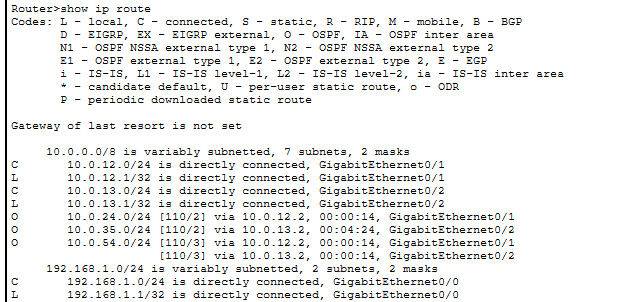
\includegraphics[width=0.7\textwidth]{figures/OSPF_show_1.png}
  \caption{OSPF路由表}
  \label{fig:jiwang}
\end{figure}

我们对FPH51\_Router0进行如下命令：int g0/1，ip ospf cost 100

通过命令，我们对该路由器cost进行了设置，然后重新回到 FPH51\_Router0使用命令show ip route查看其路由，得到下属结果：

\begin{figure}[H]
  \centering
  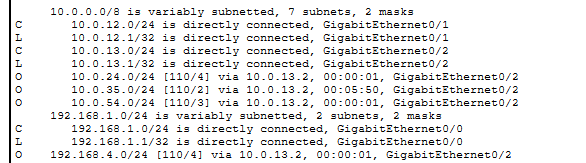
\includegraphics[width=0.7\textwidth]{figures/OSPF_show_2.png}
  \caption{OSPF路由表}
  \label{fig:jiwang}
\end{figure}

通过结果我们发现，修改cost后，OSPF直接走\ 10.0.13.2\ ，即改走长路径（R0 → R2 → R4 → R3）说明在相同拓扑条件下，配置 OSPF 动态路由协议。OSPF 能够基于接口 cost 自动计算最优路径，默认情况下选择代价较低的路径。当通过手动调整接口 cost 后，OSPF 能够重新计算路由并选择新的最优路径，体现了其较 RIP 更灵活、可控的选路机制。

\newpage

\subsubsection{综合网络情景设计}

\noindent {\heiti 网络拓扑结构与划分方案}

我们模拟学校年级办公室电脑的网络集成，功能设计如下：

\begin{itemize}
  \item 每个年级划分一个 VLAN，每个 VLAN 下包含两台 PC。
  \item 同一楼层的电脑通过二层交换机连接，不同楼层的网络通过三层交换机连接，并配置 OSPF 动态路由。
  \item 二楼是一、二年级办公室，三楼是三、四年级办公室。
  \item 设置一台内部局域网 WEB 服务器，与学校内网路由器相连。
  \item 设置一台学校外部广域网 WEB 服务器，与学校外网路由器相连。
  \item 内网路由器与外网路由器相连，通过配置 NAT 转换，使学校电脑可以通过内网访问外网。
\end{itemize}

拓扑结构设计如下，包含 8 台 PC、2 台二层交换机、1 台三层交换机、2 台路由器、2 台服务器：

\begin{figure}[H]
  \centering
  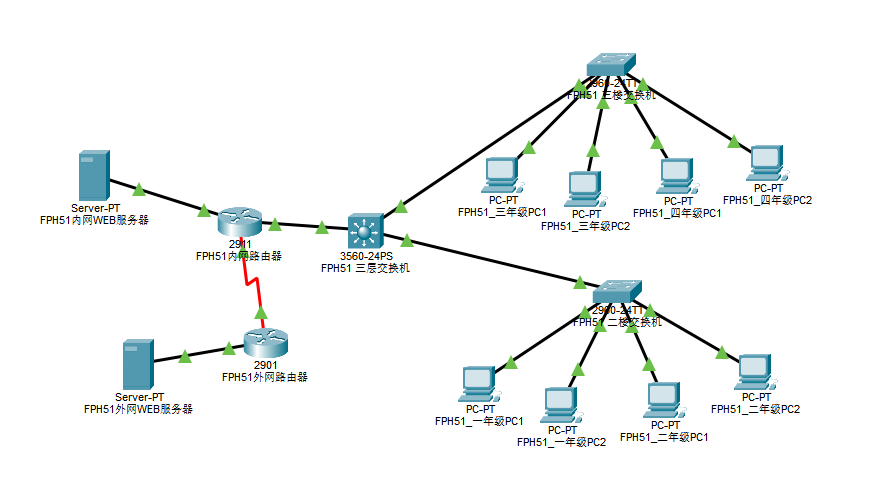
\includegraphics[width=1\textwidth]{figures/jicheng.png}
  \caption{综合网络情景设计拓扑结构}
  \label{fig:jiwang}
\end{figure}

网络划分方案如下：

\begin{table}[H]
\centering
\caption{综合网络设计实验网络地址规划表}
\renewcommand{\arraystretch}{1.2}
\begin{tabular}{ccccc}
\hline
设备名称 & 接口名称 & IP 地址 & 子网掩码 & 默认网关 \\
\hline

FPH51\_一年级PC1 & FastEthernet0 & 192.168.1.1 & 255.255.255.0 & 192.168.1.254 \\
FPH51\_一年级PC2 & FastEthernet0 & 192.168.1.2 & 255.255.255.0 & 192.168.1.254 \\

FPH51\_二年级PC1 & FastEthernet0 & 192.168.2.1 & 255.255.255.0 & 192.168.2.254 \\
FPH51\_二年级PC2 & FastEthernet0 & 192.168.2.2 & 255.255.255.0 & 192.168.2.254 \\

FPH51\_三年级PC1 & FastEthernet0 & 192.168.3.1 & 255.255.255.0 & 192.168.3.254 \\
FPH51\_三年级PC2 & FastEthernet0 & 192.168.3.2 & 255.255.255.0 & 192.168.3.254 \\

FPH51\_四年级PC1 & FastEthernet0 & 192.168.4.1 & 255.255.255.0 & 192.168.4.254 \\
FPH51\_四年级PC2 & FastEthernet0 & 192.168.4.2 & 255.255.255.0 & 192.168.4.254 \\


FPH51\ 二层交换机 & VLAN1 & 192.168.1.254 & 255.255.255.0 & — \\
FPH51\ 二层交换机 & VLAN2 & 192.168.2.254 & 255.255.255.0 & — \\
FPH51\ 二层交换机 & VLAN3 & 192.168.3.254 & 255.255.255.0 & — \\
FPH51\ 二层交换机 & VLAN4 & 192.168.4.254 & 255.255.255.0 & — \\
FPH51\ 三层交换机 & FastEthernet0/3 & 192.168.10.2 & 255.255.255.0 & — \\


FPH51\ 内网路由器 & FastEthernet0/0 & 192.168.60.254 & 255.255.255.0 & — \\
FPH51\ 内网路由器 & FastEthernet1/0 & 192.168.10.1 & 255.255.255.0 & — \\
FPH51\ 内网路由器 & Serial2/0 & 201.1.8.1 & 255.255.255.0 & — \\

FPH51\ 外网路由器 & Serial2/0 (DCE) & 201.1.8.10 & 255.255.255.0 & — \\
FPH51\ 外网路由器 & FastEthernet1/0 & 202.1.1.254 & 255.255.255.0 & — \\


FPH51\ 内网WEB服务器 & FastEthernet0 & 192.168.60.1 & 255.255.255.0 & 192.168.60.254 \\
FPH51\ 外网WEB服务器 & FastEthernet0 & 202.1.1.1 & 255.255.255.0 & 202.1.1.254 \\

\hline
\end{tabular}
\end{table}

\noindent {\heiti 相关命令介绍}

\begin{itemize}
  \item \texttt{access-list ID PERMISSION ADDR ANTIMASK}：指定访问控制列表；
  \item \texttt{ip nat}：进行 NAT 相关配置；
\end{itemize}

\noindent {\heiti 配置过程与结果分析}

设备 IP 地址的设置、交换机及路由器的基本配置我们在前面几个实验中已经详细讲解过了，在这个实验中我们不再赘述。

本实验中两个特殊的配置如下：
在进行三层交换机的端口 ip 配置时，interface fastEthernet 默认进入的是端口的二层配置，需要输入 no switchport 才能进入端口的三层进行路由相关的端口配置。

\begin{figure}[H]
  \centering
  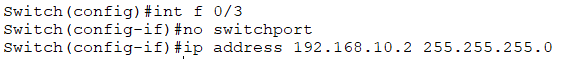
\includegraphics[width=1\textwidth]{figures/jicheng_sw.png}
  \caption{进入三层交换机的三层端口}
  \label{fig:jiwang}
\end{figure}

\newpage

\noindent\textbf{L12-内网路由器的 NAT 配置：}

\medskip
\begin{tabular}{p{7cm} p{7cm}}
\texttt{enable} & 进入特权模式 \\
\texttt{configure terminal} & 进入全局配置模式 \\

\texttt{interface fastEthernet 1/0} & 进入子接口 1/0 \\
\texttt{ip nat outside} & 配置该接口为 NAT 外部接口 \\
\texttt{exit} & 返回上一级模式 \\

\texttt{interface serial 2/0} & 进入子接口 2/0 \\
\texttt{ip nat inside} & 配置该接口为 NAT 内部接口 \\
\texttt{exit} & 返回上一级模式 \\

\texttt{access-list 1 permit 192.168.10.0 0.0.0.255} & 对 LAN 构造一个访问控制列表 \\
\texttt{ip nat pool rebmit 201.1.8.2 201.1.8.2 netmask 255.0.0.0} & 配置可用的被映射 IP 地址池 \\
\texttt{ip nat inside source list 1 pool rebmit overload} & 建立映射并配置为 NAPT \\
\texttt{end} & 返回特权模式 \\
\end{tabular}

\begin{figure}[H]
  \centering
  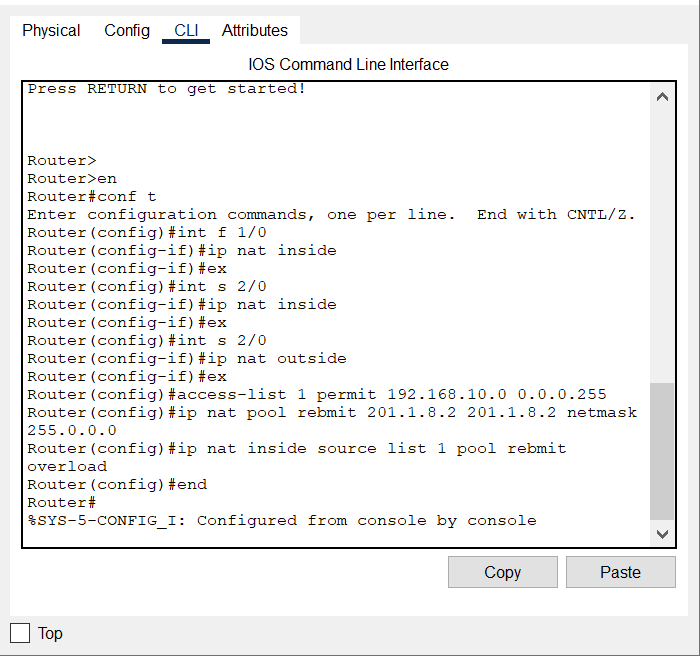
\includegraphics[width=0.7\textwidth]{figures/jicheng_inside_NAT.png}
  \caption{NAT 配置过程截图}
  \label{fig:jiwang}
\end{figure}

所有设备都配置完成后，我们来测试一下年级办公室的电脑是否能上网了。

测试结果如下：

\begin{figure}[H]
  \centering
  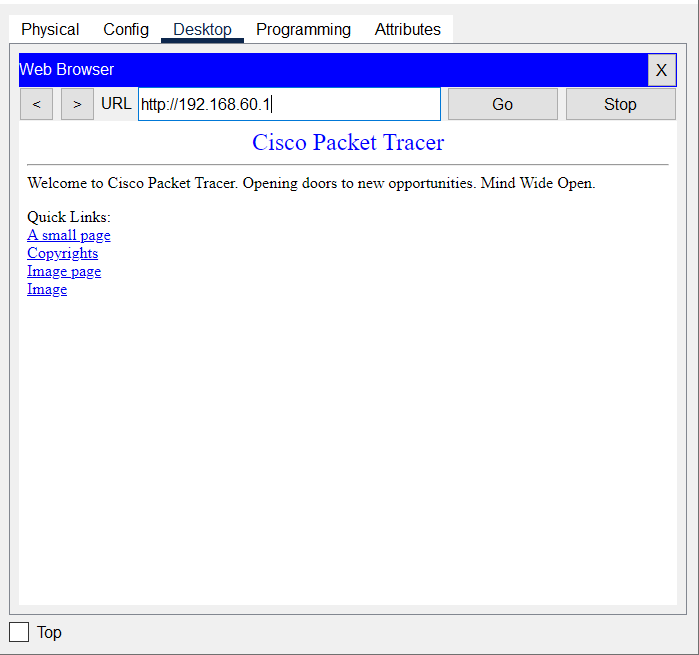
\includegraphics[width=0.7\textwidth]{figures/jicheng_test1.png}
  \caption{FPH51\_ 一年级 PC1 通过 ip 访问内网}
  \label{fig:jiwang}
\end{figure}

\begin{figure}[H]
  \centering
  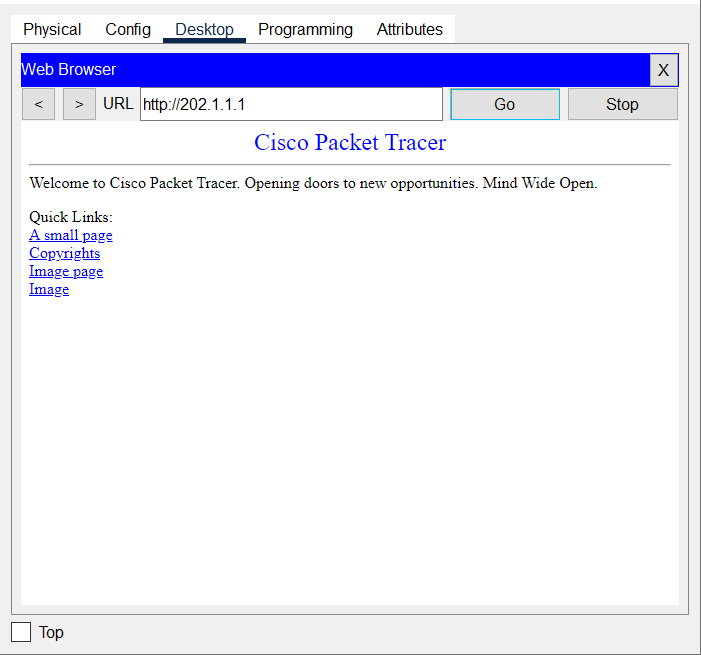
\includegraphics[width=0.7\textwidth]{figures/jicheng_test_2.png}
  \caption{FPH51\_ 一年级 PC1 通过 ip 访问外网}
  \label{fig:jiwang}
\end{figure}

\begin{figure}[H]
  \centering
  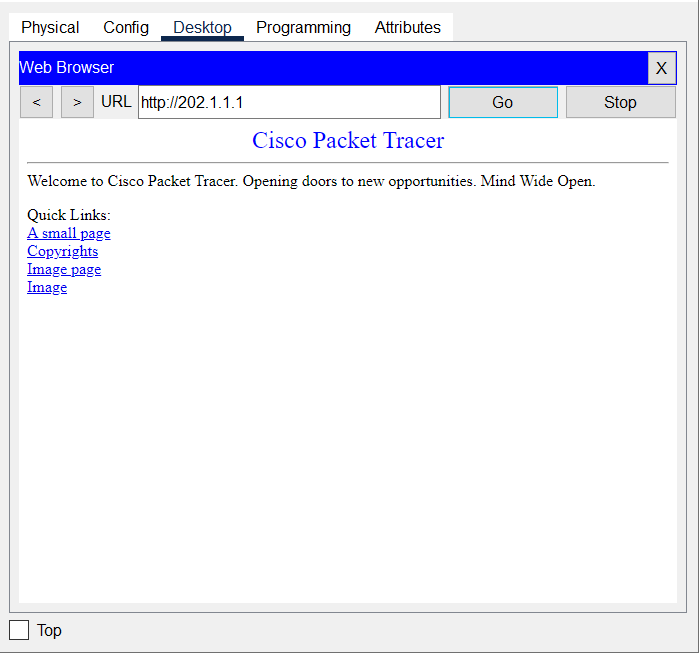
\includegraphics[width=0.7\textwidth]{figures/jicheng_test3.png}
  \caption{FPH51\_ 一年级 PC1 通过域名访问外网}
  \label{fig:jiwang}
\end{figure}

内网电脑能通过 ip 或者域名访问内网服务器、外网服务器，测试结果符合预期。

\newpage

% ---------- 2.3 网络编程 ----------

\subsection{网络编程}

\subsubsection{课程要求}

编程要求：捕获本机网卡的 IP 包，对捕获的 IP 包进行解析。要求必须输出以下字段：版本号、总长度、标识、标志位、片偏移、协议、源地址和目的地址。要有详细的说明文档，包括程序的设计思想、工作流程、关键问题、程序注释和对捕获包的解析截图。编程语言不作要求，可使用自己熟悉的 C、C++、java 或 C# 等

\subsubsection{设计思想}

实验要求捕获本机网卡的 IP 数据包，并对其进行解析，编程语言不限。基于个人对编程语言的熟悉程度，我选择用 C++ 来完成本次网络编程的编写工作。

总体需要完成的工作有两项：第一项是捕获本机网卡 IP 包，第二项是解析 IP 包。

\begin{figure}[H]
  \centering
  
\includegraphics[width=0.4\textwidth]{figures/lct1.png}
  \caption{网络编程总体设计思路}
  \label{fig:jiwang}
\end{figure}

对于第一项工作，我们需要先获得本机网卡的 ip 地址，然后使用原始套接字（raw socket）绑定该ip 地址来接收本机网卡上的数据包。

对于第二项工作，基于对 IP 数据包格式的了解，我们可以设计一个结构体指针来对 IP 数据包的头部进行逐字节的扫描解析。

\subsubsection{实验环境}

网络编程在 GCC 8.1.0 + MinGW-w64 8.1.0 环境下开发，
使用 Visual Studio Code 开发套件，以下为开发及测试平台相关信息：

\begin{itemize}
  \item 处理器：Intel(R) Core(TM) i7-14650HX (2.20 GHz)
  \item 内存：16.00GB
  \item Windows 11 家庭中文版，64 位操作系统, 基于 x64 的处理器
\end{itemize}

\newpage

\subsubsection{主要函数与结构体分析}
\noindent {\heiti 抓包函数}

这一部分使用 C++ 的 winSocks2 库实现，具体流程图如下：

\begin{figure}[H]
  \centering
  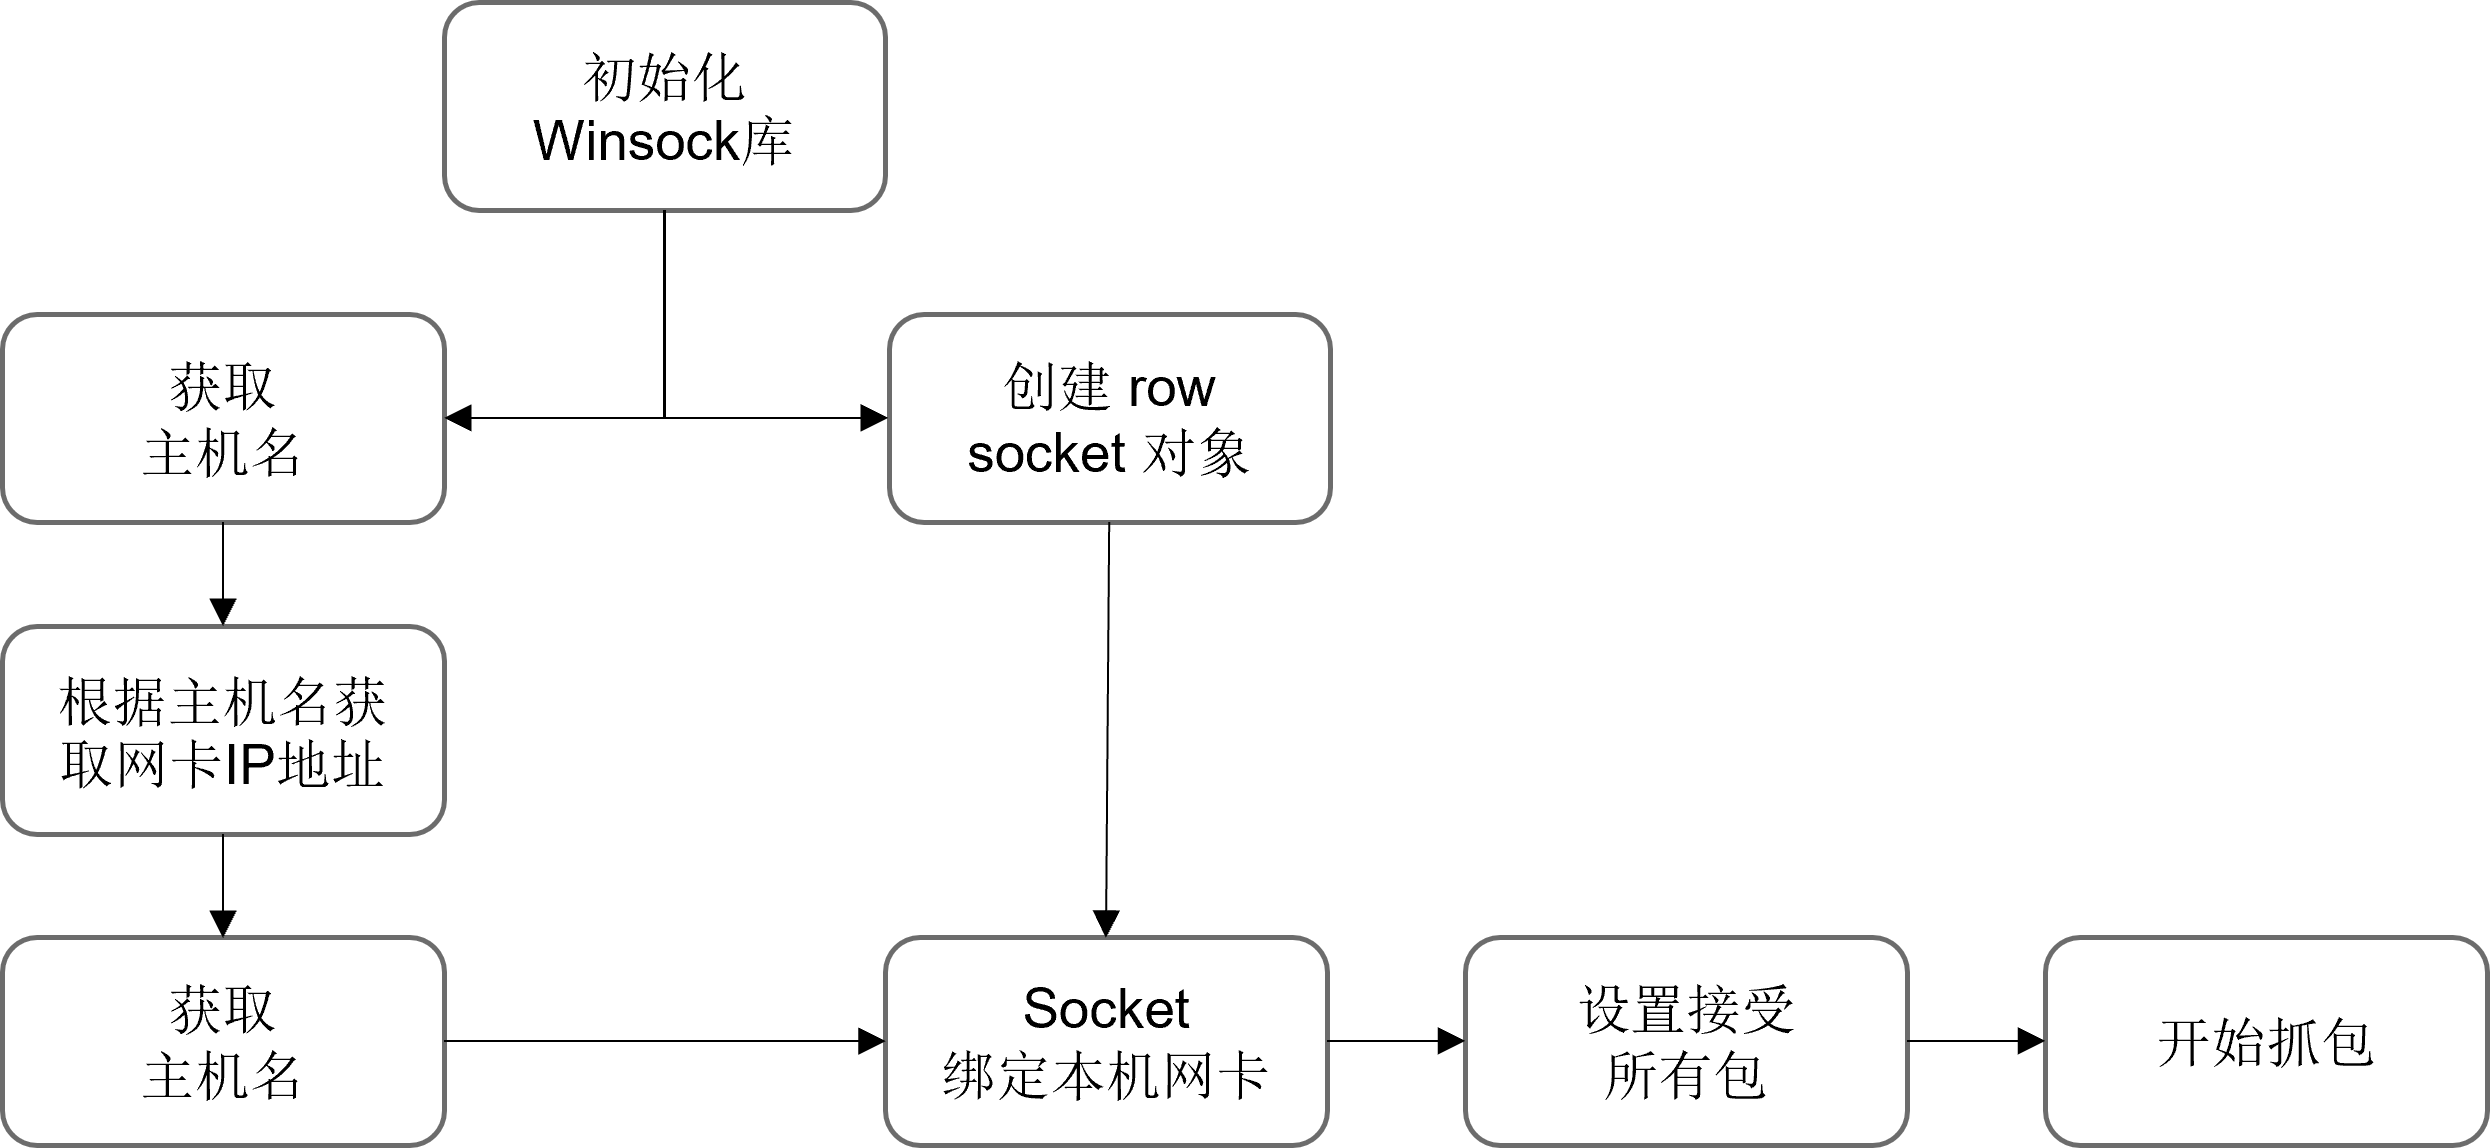
\includegraphics[width=1\textwidth]{figures/lct2.png}
  \caption{抓包流程图}
  \label{fig:jiwang}
\end{figure}

通过查阅文档，我们了解到了相应库函数的使用方式：

\begin{itemize}
  \item 初始化 winsock 库：
\begin{lstlisting}
WSAStartup(0x0202, &wsa_data);
\end{lstlisting}

  \item 获取主机名：
\begin{lstlisting}
gethostname(hostname, maxHostNameLen);
\end{lstlisting}

  \item 根据主机名获取网卡 IP 地址：
\begin{lstlisting}
HOSTENT *host = gethostbyname(hostname);
\end{lstlisting}

  \item 创建 \texttt{SOCKADDR\_IN} 对象：
\begin{lstlisting}
SOCKADDR_IN address{};
address.sin_addr.s_addr = *(unsigned long *)host->h_addr;
address.sin_family = AF_INET;
address.sin_port = htons(0);
\end{lstlisting}

  \item 创建 raw socket 对象：
\begin{lstlisting}
SOCKET sockServer = socket(AF_INET, SOCK_RAW, IPPROTO_IP);
\end{lstlisting}

  \item 绑定本机网卡：
\begin{lstlisting}
bind(sockServer, (SOCKADDR *)&address, sizeof(SOCKADDR));
\end{lstlisting}

  \item 设置接收所有数据包：
\begin{lstlisting}
WSAIoctl(sockServer, SIO_RCVALL,
          &dwInBuff, sizeof(dwInBuff),
          &dwOutBuff, sizeof(dwOutBuff),
          &dwBytesRet, nullptr, nullptr);
\end{lstlisting}

  \item 开始抓包：
\begin{lstlisting}
recv(sockServer, buffer, maxBufferSize, 0);
\end{lstlisting}
\end{itemize}

\noindent {\heiti 头部扫描结构体}

该结构体用于解析 IP 数据报头部，不考虑选项字段，默认头部长度为 20 字节。

基于 IP 头部字段顺序，我们设计了如下结构体：

\begin{lstlisting}
struct IP_datagram {
    unsigned char Version_IHL;        // 版本 4 位 + 首部长度 4 位
    unsigned char TOS;                // 服务类型
    unsigned short TL;                // 总长度
    unsigned short id;                // 标识
    unsigned short flags_fragOffset;  // 标志位 3 位 + 片偏移 13 位
    unsigned char TTL;                // 生存时间
    unsigned char protocol;           // 协议
    unsigned short headerChecksum;    // 首部校验和
    unsigned int srcAdd;              // 源地址
    unsigned int destAdd;             // 目的地址
};
\end{lstlisting}

为了便于输出字段的含义，我们设计了若干解析函数。

\paragraph{协议字段解析函数}

\begin{lstlisting}
std::string getProtocol() const {
    switch (protocol) {
        case 1:  return "ICMP (1)";
        case 2:  return "IGMP (2)";
        case 6:  return "TCP (6)";
        case 17: return "UDP (17)";
        default: return std::to_string((int)protocol);
    }
}
\end{lstlisting}

\paragraph{IP 版本解析函数}

\begin{lstlisting}
std::string getVersion() const {
    unsigned char version = Version_IHL >> 4;
    switch (version) {
        case 4: return "IPv4 (4)";
        case 6: return "IPv6 (6)";
        default: return std::to_string((int)version);
    }
}
\end{lstlisting}

\paragraph{标志位解析函数}

\begin{lstlisting}
std::string getFlag() const {
    unsigned char flags = flags_fragOffset >> 13;
    std::string description;
    if (flags & 0b001) description += "more fragments, ";
    if (flags & 0b010) description += "don't fragment, ";
    if (description.empty()) return "0";
    description.pop_back();
    description.pop_back();
    description += " (" + std::to_string(flags) + ")";
    return description;
}
\end{lstlisting}

\newpage
\subsubsection{程序流程图}
程序完整流程图如下：

\begin{figure}[H]
  \centering
  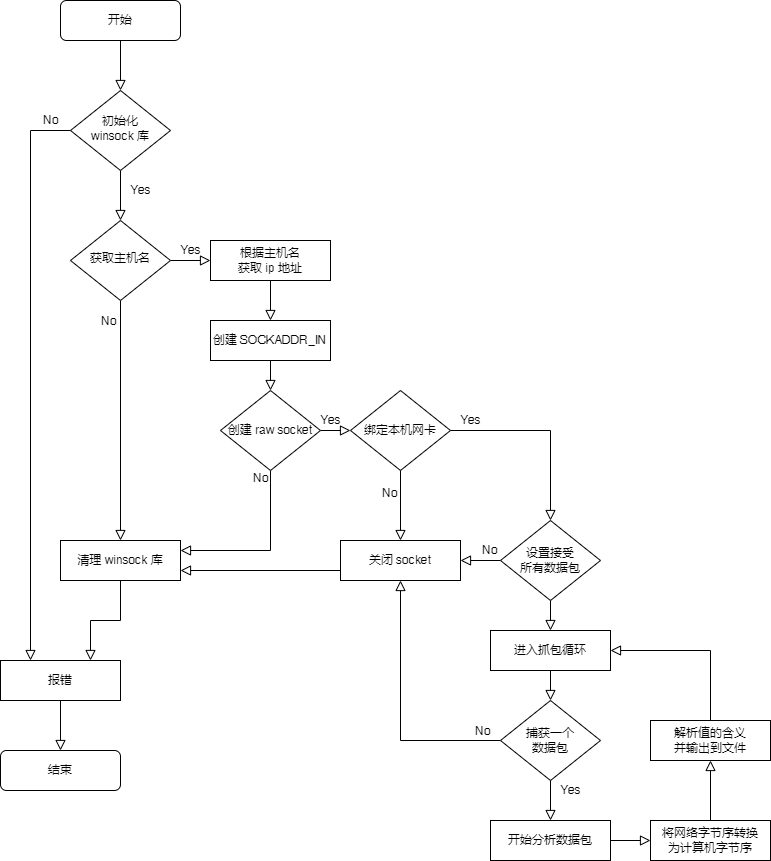
\includegraphics[width=1\textwidth]{figures/lct3.png}
  \caption{程序完整流程图}
  \label{fig:jiwang}
\end{figure}

\subsubsection{难点解决}

进行课程设计过程中遇到的难点主要有以下三个：

\noindent {\heiti 编译链接}

在使用 winsock2 库头文件时，编译器报错找不到相应的库文件。

通过查阅资料，winsock2 作为动态链接库，在用 CMake 编译时，需要在 CMakeLists 中加入target\_link\_libraries(PacketCapture WS2\_32) ，若使用 GCC 编译则需要在编译命令后加上参数 -lWS2\_32。

\noindent {\heiti 管理员权限}

刚开始进行抓包函数编写的时候，绑定网卡的函数 bind() 一直返回错误信息，经过查阅资料，得知 windows 下进行 socket 的绑定需要管理员权限。

用管理员权限打开 cmd 再进行编译操作即可解决。

\noindent {\heiti 字节序问题}

在写好 IP\_datagram 结构体进行初步测试时，我们发现解析得到结果不太正常，具体表现有 IP报的版本都不是 IPv4 和 IPv6，协议解析不出等。

通过查阅资料，我们了解到网络字节序与计算机字节序的差异，在大于 1 个字节的字段处理上，需要注意二者的转换。
最终我们用 winsock2 库提供的 htons、htonl、ntohs、ntohl 用于字节序转换的函数解决了这个问题。

\subsubsection{测试结果截图}
我们对\ main.cpp\ 文件进行编译得到main.exe，接着以管理员身份运行该文件，未出现报错信息，得到运行过程如下：

\begin{figure}[H]
  \centering
  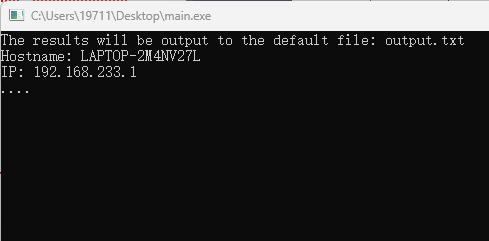
\includegraphics[width=1\textwidth]{figures/zhuabao.png}
  \caption{抓包过程截图}
  \label{fig:jiwang}
\end{figure}

每输出一个点表示成功抓到了一个包。当抓到的包数量足够多后，我们用 Ctrl + C 中断程序停止抓包。

我们可以看到当前目录下多了 output.txt 输出文件，点开里面是解析好的 IP 数据包信息。

\begin{figure}[H]
  \centering
  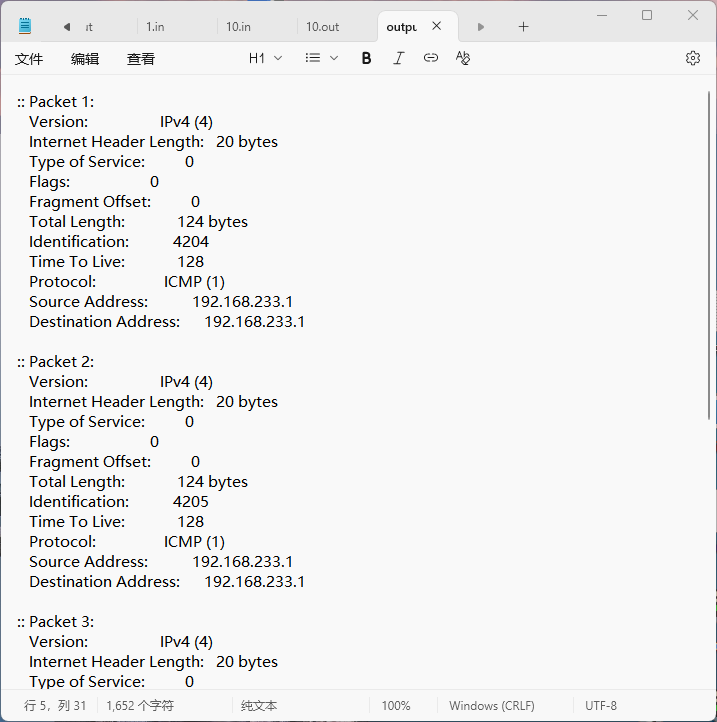
\includegraphics[width=1\textwidth]{figures/output.png}
  \caption{output.txt文件}
  \label{fig:jiwang}
\end{figure}

输出结果包含了版本号、总长度、标识、标志位、片偏移、协议、源地址和目的地址，符合实验要求。

\subsubsection{实验结果分析}

接下来我们节选一个输出片段进行分析：

\begin{verbatim}
:: Packet 1:
   Version:                  IPv4 (4)
   Internet Header Length:   20 bytes
   Type of Service:          0
   Flags:                    0
   Fragment Offset:          0
   Total Length:             124 bytes
   Identification:           4204
   Time To Live:             128
   Protocol:                 ICMP (1)
   Source Address:           192.168.233.1
   Destination Address:      192.168.233.1
\end{verbatim}

分析：

\begin{itemize}
  \item 抓到的数据报为 IPv4 数据报。
  \item 首部长度字段值为 5，对应 20 字节，说明该数据报未携带 IPv4 可选字段。
  \item 服务类型字段为 0，表示使用默认的服务质量。
  \item 标志位为 0，说明该数据报未被设置分片相关标志。
  \item 片偏移量为 0，表示该数据报未发生分片。
  \item 数据报总长度为 124 字节，包含 IPv4 首部与上层协议数据。
  \item 标识字段值为 4204，用于在发生分片时对数据报进行重组。
  \item 生存时间（TTL）为 128，说明该数据报最多可经过 128 跳路由器转发。
  \item 上层协议类型为 ICMP，对应协议号为 1。
  \item 源地址与目的地址均为 192.168.233.1，说明该 ICMP 数据报为主机本地发起并接收的数据包，常见于本地连通性测试。
\end{itemize}

\subsubsection{程序源代码}

下面给出本实验所实现的完整程序源代码，采用 C++ 语言编写，基于 Windows 平台的 raw socket 机制实现 IP 数据包的捕获与解析。

\begin{lstlisting}[language=C++,caption={IP 数据包捕获与解析程序源码}]
#include <bits/stdc++.h>

// raw socket 编程所需头文件，需要链接到动态库 WS2_32
#include <winsock2.h>
#include <mstcpip.h>

const char *const filePath = "output.txt";
const int maxHostNameLen = 256;     // 8 位
const int maxBufferSize  = 65536;  // 16 位

char buffer[maxBufferSize];

struct IP_datagram {
    unsigned char Version_IHL;        // 版本 4 位 + 首部长度 4 位
    unsigned char TOS;                // 服务类型
    unsigned short TL;                // 总长度
    unsigned short id;                // 标识
    unsigned short flags_fragOffset;  // 标志位 3 位 + 片偏移 13 位
    unsigned char TTL;                // 生存时间
    unsigned char protocol;           // 协议
    unsigned short headerChecksum;    // 首部校验和
    unsigned int srcAdd;              // 源地址
    unsigned int destAdd;             // 目的地址

    std::string getProtocol() const {
        switch (protocol) {
            case 1:  return "ICMP (1)";
            case 2:  return "IGMP (2)";
            case 6:  return "TCP (6)";
            case 17: return "UDP (17)";
            default: return std::to_string((int)protocol);
        }
    }

    std::string getVersion() const {
        unsigned char version = Version_IHL >> 4;
        switch (version) {
            case 4: return "IPv4 (4)";
            case 6: return "IPv6 (6)";
            default: return std::to_string((int)version);
        }
    }

    std::string getFlag() const {
        unsigned char flags = flags_fragOffset >> 13;
        std::string description;
        if (flags & 0b001) description += "more fragments, ";
        if (flags & 0b010) description += "don't fragment, ";
        if (description.empty()) return "0";
        description.pop_back();
        description.pop_back();
        description += " (" + std::to_string(flags) + ")";
        return description;
    }

    void invertByte() {
        unsigned short inv[10];
        unsigned short *p = (unsigned short *)this;
        for (int i = 0; i < 10; i++) {
            memcpy(inv + i, p, sizeof(unsigned short));
            if (i == 1 || i == 2 || i == 3 || i == 5)
                inv[i] = ntohs(inv[i]);
            p++;
        }
        memcpy(this, inv, sizeof(unsigned short) * 10);
    }
};

static int count = 0;

void analyze(char *buffer, int length) {
    auto *ip = (IP_datagram *)buffer;
    ip->invertByte();
    SOCKADDR_IN address{};

    printf(":: Packet %d:\n", count);
    printf("   Version:                  %s\n", ip->getVersion().c_str());
    printf("   Internet Header Length:   %d bytes\n",
           (ip->Version_IHL & 0b00001111) * 4);
    printf("   Type of Service:          %d\n", ip->TOS);
    printf("   Flags:                    %s\n", ip->getFlag().c_str());
    printf("   Fragment Offset:          %d\n",
           ip->flags_fragOffset & 0b0001111111111111);
    printf("   Total Length:             %d bytes\n", ip->TL);
    printf("   Identification:           %d\n", ip->id);
    printf("   Time To Live:             %d\n", ip->TTL);
    printf("   Protocol:                 %s\n", ip->getProtocol().c_str());

    address.sin_addr.s_addr = ip->srcAdd;
    printf("   Source Address:           %s\n",
           inet_ntoa(address.sin_addr));
    address.sin_addr.s_addr = ip->destAdd;
    printf("   Destination Address:      %s\n",
           inet_ntoa(address.sin_addr));

    puts("");
}

int captureData() {
    WSAData wsa_data{};
    char hostname[maxHostNameLen];

    DWORD dwInBuff = 1;
    DWORD dwOutBuff;
    DWORD dwBytesRet;

    if (WSAStartup(0x0202, &wsa_data)) {
        fprintf(stderr, "WSA startup failed.\n");
        return -1;
    }

    if (gethostname(hostname, maxHostNameLen)) {
        fprintf(stderr, "Failed to get hostname.\n");
        WSACleanup();
        return -1;
    }

    HOSTENT *host = gethostbyname(hostname);

    SOCKADDR_IN address{};
    address.sin_addr.s_addr = *(unsigned long *)host->h_addr;
    address.sin_family = AF_INET;
    address.sin_port = htons(0);

    SOCKET sockServer = socket(AF_INET, SOCK_RAW, IPPROTO_IP);
    if (sockServer < 0) {
        WSACleanup();
        return -1;
    }

    if (bind(sockServer, (SOCKADDR *)&address, sizeof(SOCKADDR))) {
        closesocket(sockServer);
        WSACleanup();
        return -1;
    }

    if (WSAIoctl(sockServer, SIO_RCVALL,
                 &dwInBuff, sizeof(dwInBuff),
                 &dwOutBuff, sizeof(dwOutBuff),
                 &dwBytesRet, nullptr, nullptr)) {
        closesocket(sockServer);
        WSACleanup();
        return -1;
    }

    while (true) {
        memset(buffer, 0x00, sizeof(buffer));
        int bufferSize = recv(sockServer, buffer, maxBufferSize, 0);
        if (bufferSize < 0) break;
        ++count;
        analyze(buffer, bufferSize);
    }

    closesocket(sockServer);
    WSACleanup();
    return 0;
}

int main(int argc, char *argv[]) {
    if (argc == 1) {
        freopen(filePath, "w", stdout);
    } else if (argc == 2) {
        freopen(argv[1], "w", stdout);
    } else {
        return -1;
    }
    return captureData();
}
\end{lstlisting}


% =================================================
% 三、课程设计总结体会
% =================================================

\newpage
\section{课程设计总结体会}

通过本次计算机网络课程设计，我对课堂上所学习的网络基础知识有了更加系统和深入的认识。从最初对网络结构和设备功能理解不够清晰，到能够独立完成网络拓扑的搭建与配置，我逐步体会到了理论知识在实际应用中的重要性。在实验过程中，我熟练掌握了如 ping、ipconfig、tracert、show ip route 等常用网络命令的使用方法，并能够通过命令输出来分析网络的连通性和故障原因。同时，我对交换机和路由器的基本配置流程有了清晰的认识，包括设备初始化、接口配置、VLAN 划分以及路由设置等内容。

在综合网络情景设计部分，我将所学的网络原理与实际操作相结合，围绕多 VLAN 环境下的通信需求完成了整体网络的规划与实现。在查阅和整理大量相关资料的基础上，我成功配置了三层交换机与路由器的互联，并通过动态路由协议实现了各个网络之间的通信。此外，在内外网隔离的实验环境中，通过在出口路由器上配置 NAT 技术，使内网主机能够正常访问外网服务器，从而加深了我对地址转换原理及其应用场景的理解。在此过程中，我还完成了 WEB 和 DNS 服务器的基本配置，对服务器在网络中的作用和工作方式有了更加直观的认识。

在网络编程部分，我初步接触并学习了基于 Socket 的网络编程方法，通过编写程序实现了简单的数据抓包功能。通过对捕获到的数据进行分析，我能够将课堂上所讲的 IP 数据报结构、协议字段等知识与实际数据对应起来，加深了对网络数据传输过程的理解。这一过程不仅提升了我的动手能力，也让我体会到理论与实践相结合所带来的学习效果和成就感。

总体而言，本次课程设计内容完整、实践性强，使我在网络设备配置、综合网络设计以及网络编程等多个方面都得到了锻炼和提升。通过不断调试和排错，我的分析问题和解决问题的能力也得到了明显增强。这次课程设计让我受益匪浅，为今后参与实际项目开发以及进行复杂网络环境的配置和维护打下了良好的基础。

\end{document}
